
The actin cortex is a thin layer ($\sim0.2 \si{\micro \meter}$ in thickness for a typical
cell radius of $\sim 10 \si{\micro \meter}$) of a crosslinked network of actin filaments undergoing turnover and actively driven by ATP hydrolysis \cite{chugh2018}. This network can self-organize into dense and highly ordered structures as a result of out-of-equilibrium force generation by  bundling proteins \cite{cortes2018, leite2019,turlier2014} and self-reinforcing flows \cite{khaliullin2018}. These nematic assemblies exert in-plane as well as out-of-plane anisotropic contractile tensions on the curved surface of the cell \cite{cortes2018, leite2019,kelkar2020}, leading to cell elongation and to splitting of a cell into two daughter cells during cytokinesis \cite{turlier2014, turlier2021}.
%or a vesicle forming furrow-like indentations \cite{litschel2021}. 
Different physical aspects of cytokinesis have been studied using either agent-based models \cite{pinto2012, bidone2014, bidone2017} or continuum models based on partial differential equations \cite{greenspan1978, mietke2019_2, mietke2019, koyama2012,gladilin2015,biron2005,salbreux2009,turlier2014,sain2015,zhao2016}. Such continuum surface active gel models have also been used to understand amoeboid cell motility \cite{callan2013,lim2013,Ruprecht:2015aa,lee2018,torres2019,moreno2020, wang2021}. Each of these models makes different assumptions about the mechanical nature of the cortical material, including interfacial viscous fluids with \cite{greenspan1978, mietke2019_2, mietke2019} or without \cite{turlier2014,torres2019,biron2005,sain2015,zhao2016} bending rigidity, purely elastic membranes \cite{koyama2012,gladilin2015}, or viscoelastic membranes \cite{akkacs1980,poirier2012}. The process of cell division happens on timescales of minutes, significantly longer than those of turnover ($\sim 0.1 \si{\second}^{-1}$), which suggests that the elastic response of the network  can be ignored in this context  \cite{salbreux2009}.


The onset of cell division is driven by equatorial myosin activation, which drives cortical flows from the poles towards the equator \cite{spira2017}. During this process, velocity gradients produce network alignment, which further enhances contractility in the equatorial region in a self-reinforcing process \cite{anne2016}. To the best of our knowledge, this is the only reference that has accounted, with important simplifications, for the establishment and mechanical influence of network alignment during cytokinesis. Here, we particularize the model for an active nematic  gel on deformable surfaces developed in Chapter~\ref{chap_7} to axisymmetry, pertinent to cell division, and formulate and implement a computational finite element method to solve the governing equations in the fully nonlinear regime. Following observations \cite{spira2017} and in agreement with previous work \cite{turlier2014}, we trigger cytokinesis with an equatorial over-activity. We find that, as compared to previously studied isotropic active gel models \cite{turlier2014},  the nematic coupling enables a faster and much more efficient mechanism of cytokinesis requiring smaller over-activities. In the absence of over-activity, linear stability analysis shows that an isotropic and uniform active gel layer on a spherical surface can develop cytokinetic-like dynamical modes \cite{mietke2019_2}, suggesting that during cytokinesis the biologically regulated equatorial activation may act in concert with the ability of the cortex to self-organize. Our nonlinear simulations suggest, however, that this symmetry-breaking mode becomes unstable and transits to a polarize ``cell motility'' mode in the absence of nematic coupling. Instead, the cytokinetic-like spontaneous symmetry-breaking mode remains stable and leads to full cleavage in the present model. 
 
 The chapter is organized as follows. Section~\ref{2_3_1} describes the kinematics of an axisymmetric surface, as well as the calculation of covariant and Lie derivatives of fields on the surface. In Section~\ref{Rayl_axi}, we particularize the general Rayleighian developed in the previous chapter to the axisymmetric setting and to a Lagrangian description of motion. In Section~\ref{2_3_2}, we first discretize the problem in time by introducing a time-incremental Rayleighian functional. We then introduce the finite element space discretization using B-Spline basis functions and derive the discrete algebraic equations governing the evolution of position, nematic order and density from the time-incremental Onsager variational principle. We also describe the reparametrization of the generating curve required to avoid excessive mesh distortions in our Lagrangian description of motion.  In Section~\ref{2_3_3}, we apply the numerical solution of the axisymmetric model to examine physical aspects of cell division.

\section{Kinematics of an axisymmetric surface} \label{2_3_1}

We parametrize the axisymmetric surface $\Gamma$ embedded in three-dimensional space as 
\begin{equation}  \label{1_III}
    \bm{x}(u,\varphi) = (r(u)\textup{cos} \varphi, r(u) \textup{sin} \varphi, z(u)),
\end{equation}
where $u \in [0,1]$ is the parametric coordinate of the generating curve $\mathcal{C}$ given by the functions $r(u)$ and $z(u)$, and $\varphi \in [0,2\pi]$ is the angle about the $z-$axis, Fig.~\ref{fig_2}(a).  Due to the assumption of axisymmetry, neither shape nor any other field depends on $\varphi$.  The natural tangent basis vectors associated to this parametrization are
\begin{equation} \label{2_III}
    \bm{e}_{u} = \frac{\partial \bm{x}}{\partial u} = (r'(u)\textup{cos} \varphi, r'(u) \textup{sin} \varphi, z'(u)), \;\;\;\;\;
    \bm{e}_{\varphi} = \frac{\partial \bm{x}}{\partial \varphi} = (-r(u)\textup{sin} \varphi, r(u) \textup{cos} \varphi, 0).
\end{equation}
\begin{figure}
\centering
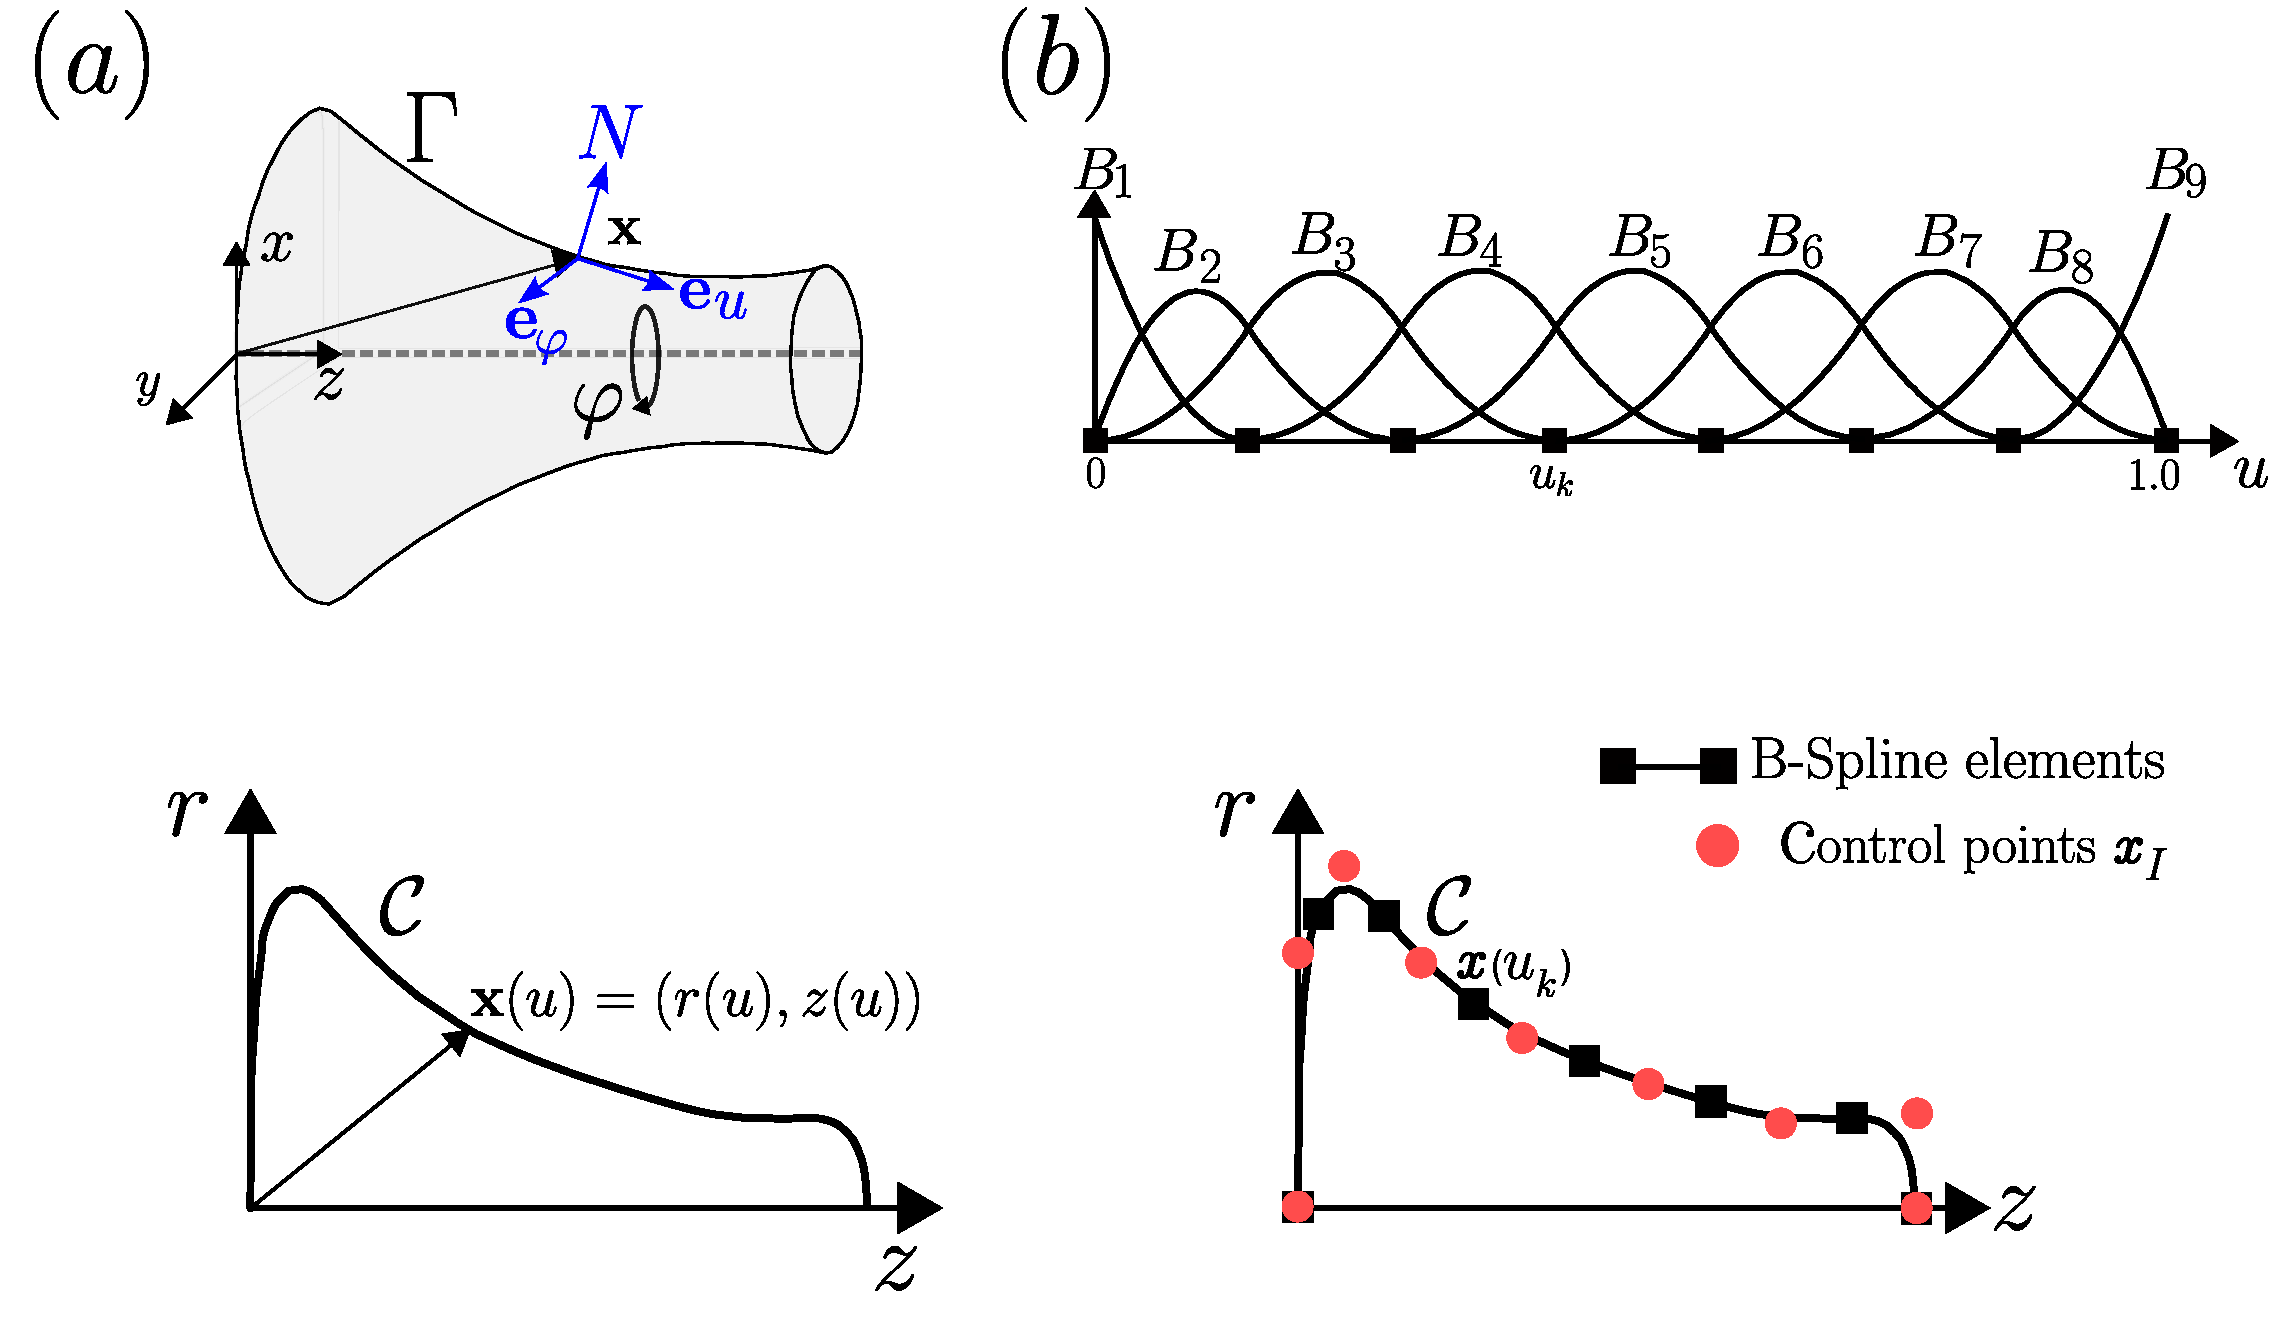
\includegraphics[width=1\textwidth]{chap_8_fig_1.pdf}
\caption{ \textbf{Kinematics and numerical approximation of an axisymmetric surface} (a) Schematic of an axisymmetric surface $\Gamma$ of revolution (top), and its representation in terms of the generating curve $\mathcal{C}$ in the $r-z$ plane (bottom). (b) Finite element approximation of an axisymmetric surface $\Gamma$ using clamped second order B-Spline basis functions $B_{I}$ and control points $\bm{x}_I$. }
\label{fig_2}
\end{figure} 
The unit normal $\bm{N}$ to the surface $\Gamma$ can be written as
\begin{equation} \label{4_III}
    \bm{N} = \frac{\bm{e}_u \times \bm{e}_\varphi}{\left|\bm{e}_u \times \bm{e}_\varphi \right|}= \frac{1}{a}(-z' \textup{cos}\varphi , -z' \textup{sin}\varphi, r'),
\end{equation}
where $a^2 = (r')^2 + (z')^2$ and we omit the explicit dependence of
$r$, $z$ and $a$ on $u$. Using Eq.~(\ref{eq::metric}). The metric tensor and its inverse are given by
\begin{equation} \label{5_III}
\{g_{ab} \} = \begin{pmatrix}
a^2 & 0 \\ 
0 & r^2 
\end{pmatrix} , \quad  \{g^{ab} \} = \begin{pmatrix}
\frac{1}{a^2} & 0 \\ 
0 & \frac{1}{r^2} 
\end{pmatrix}.
\end{equation}
The determinant of the metric tensor is  $g=\textup{det}(\bm{g}) = a^2 r^2$. Eq.~(\ref{3_II}), combined with Eqs.~(\ref{2_III}-\ref{4_III}), allows us to compute the second fundamental form as
\begin{equation} \label{6_III}
   \{k_{ab}\}= \frac{1}{a}\begin{pmatrix}
b & 0 \\ 
0 & r z'
\end{pmatrix},
\end{equation}
where $b=r'z''-r''z'$. The mean curvature  $H =k_{ab}g^{ab}$ is then
\begin{equation} \label{23_III}
	H  = \frac{1}{a}\left(\frac{b}{a^2} + \frac{z'}{r}\right).  
\end{equation}
 To compute covariant derivatives of vector and tensor fields, we require the Christoffel symbols. Using Eq.~(\ref{8_II}), they can be written explicitly as
\begin{equation} \label{7_III}
\{\Gamma^u_{~ab}\} =  \begin{pmatrix}
a'/a &0 \\ 
0 &-rr'/a^2 
\end{pmatrix}  , \quad \{\Gamma^\varphi_{~ab}\} =   \begin{pmatrix}
0 &r'/r \\ 
r'/r &0 
\end{pmatrix} ,
\end{equation}
where $a' = (r' r''+z'z'')/a $.
To consider a dynamical surface, the functions parametrizing the generating curve also depend on time, $r(u,t)$ and $z(u,t)$, and hence $\bm{x}(u,\varphi,t)$. Adopting a Lagrangian description, according to which a point $(u,\varphi)\in [0,1]\times[0,2\pi]$ labels a material particle throughout the time evolution, the Lagrangian velocity field can be expressed as 
\begin{equation}   \label{8_III}
     \bm{V}(u,\varphi,t) = \frac{\partial \bm{x}}{\partial t} (u,\varphi,t).
\end{equation}
In fact, we only need the velocity field in the $r-z$ plane, which is given by 
\begin{equation}   \label{8_III}
     \bm{V}(u,t) = \begin{pmatrix}
     	\frac{\partial r}{\partial t} (u,t)\\ 
     	\frac{\partial z}{\partial t} (u,t)
     \end{pmatrix} 
     = 
     \begin{pmatrix}
     	\dot{r} (u,t)\\ 
     	\dot{z} (u,t)
     \end{pmatrix}, 
\end{equation}
where dots denote partial time differentiation. The rate of deformation tensor $\bm{d}$ can be calculated as
\begin{equation}  \label{11_III}
\bm{d} = \frac{1}{2} \mathcal{L}_{\bm{V}} \bm{g}= \frac{1}{2} \frac{\partial  \bm{g}}{\partial t}, 
\end{equation}
where $\mathcal{L}_{\bm{V}}$ denotes the Lie derivative along the flow with velocity $\bm{V}$ \cite{marsden1994}. Because our parametrization of motion is Lagrangian, the Lie derivative can be simply computed as a partial time derivative. 

In an axisymmetric setting, we assume that the average molecular alignment $\bm{n}$ can either be  along $\bm{e}_u$ or along $\bm{e}_\varphi$. Hence,  the off-diagonal components of the nematic order tensor $q(u)$ are zero and we can express it as
\begin{equation} \label{24_III}
  \{ q^{ab} \} = \begin{pmatrix}
q^{uu} &0 \\ 
0 & q^{\varphi \varphi}
\end{pmatrix} =  \begin{pmatrix}
q &0 \\ 
0 & -  (g_{uu}/g_{\varphi \varphi}) q
\end{pmatrix}=  \begin{pmatrix}
q &0 \\ 
0 & - (a^2/r^2) q 
\end{pmatrix}, 
\end{equation}
where  we have used the fact that  $\textup{tr}~\bm{q}=0$ to represent the tensor in terms of a single scalar function $q(u,t)$.

The covariant derivative of the nematic order tensor can then be written in the axisymmetric setting as
\begin{align}  \label{13_III}
    \{\nabla_u q^{ab}\} & = \begin{pmatrix}   q'+ 2q \Gamma^u_{uu} & 0  \\
0 &  -[(g_{uu}/g_{\varphi \varphi}) q]' - 2(g_{uu}/g_{\varphi \varphi}) q \Gamma^\varphi_{\varphi u}  \end{pmatrix} \, \, , \, \, \{\nabla_\varphi q^{ab}\} = \bm{0}.  \\
& = \begin{pmatrix}   q'+ 2\frac{a'}{a} q  & 0  \\
0 &  - \frac{a^2}{r^2} q' - \frac{2 a a'}{r^2} q    \nonumber   
\end{pmatrix}.
\end{align}
The components of the Jaumann derivative of the nematic order tensor are 
\begin{align}  \label{14_III}
    \{\widehat{q}^{ab}\}  & = \begin{pmatrix}
\mathcal{L}_{\bm{V}} q + 2d^{u}_{~u}q & 0  \\
0 &  - \mathcal{L}_{\bm{V}} [(g_{uu}/g_{\varphi \varphi}) q] - 2d^{\varphi}_{~\varphi}(g_{uu}/g_{\varphi \varphi}) q 
\end{pmatrix} \\
 & = \begin{pmatrix}
\dot{q} + 2d^{u}_{~u}q & 0  \\
0 &  - \partial_t[(a^2/r^2) q] - 2d^{\varphi}_{~\varphi}(a^2/r^2) q 
\end{pmatrix}, \nonumber
\end{align}
where again the Lie derivative can be computed as a partial derivative with respect to time. 


Finally, we note that the density field only depends on $u$ and $t$ as well, $\rho = \rho(u,t)$. 

\section{Rayleighian in the axisymmetric setting} \label{Rayl_axi}

The free-energy of the system introduced in the previous chapter can then be expressed in the axisymmetric setting as
\begin{align} \label{F_axi}
   \mathcal{F}[q, r, z, \rho] = \underset{\Gamma}{\int} f \rho \,d A  = 2\pi \int_0^1 f \rho a r du,
\end{align}
where $f = f_{\rm bend} +  f_{\rm sus} +  f_{\rm frank}$ can be directly computed from Eqs.~(\ref{13_III},\ref{23_III},\ref{24_III}). Likewise, the dissipation potential
\begin{align} 
   \mathcal{D}\left[\dot{q},\dot{r},\dot{z}; q, r, z, \rho \right] = 
 2\pi \int_0^1 \bigg [  \eta \bigg(  \vert \bm{d}\vert^2 + \left(\text{tr} \, \bm{d}\right)^2\bigg) +   \frac{\eta_{\text{rot}}}{2}  \vert\widehat{\bm{q}}\vert^2 +  \beta  \bm{d}^{\rm dev}:\widehat{\bm{q}}   +  \frac{\gamma}{2} \vert\bm{V}\vert^2 \bigg]  \rho a r du   
\end{align}
and the power input 
 \begin{align}  
  \mathcal{P} \left[\dot{q},\dot{r},\dot{z}; q, r, z, \rho \right]  = 2\pi \int_0^1  \bigg[ g(\rho)\lambda \text{tr}\bm{d} +  g(\rho)\lambda_{\rm aniso}  \bm{q}\cddot \bm{d} -   h(\rho)\lambda_{\bigodot}  \bm{q} \cddot \widehat{\bm{q}}  \bigg] \rho a r du,
\end{align}
can be directly computed from Eqs.~(\ref{11_III},\ref{24_III},\ref{14_III},\ref{8_III}).
Minimization of the Rayleighian functional $d \mathcal{F}/dt + \mathcal{D} + \mathcal{P}$, possibly subject to constraints like fixed enclosed volume for a vesicle or cell, provides the Euler-Lagrange governing equations encoding balance of generalized force power conjugate to changes in nematic order, and balance of linear momentum along the $r$ and $z$ directions. 

We recall that balance of mass provides an evolution equation for  density 
\begin{equation}  \label{89_II_8}
    \dot{\rho} + \rho d_{~ a}^a   - D \Delta\rho=  s,
\end{equation}
where $\Delta$ is the surface Laplacian and $s$ is a source term, which is usually expressed as $s = -k_d(\rho-\rho_0)$, with $k_d$ the depolymerization rate, to model cytoskeletal turnover. 


\section{Axisymmetric finite element formulation based on an incremental Onsager principle} \label{2_3_2}

Rather than deriving the axisymmetric Euler-Lagrange from the variational principle, or adapting the general governing equations of the previous chapter to axisymmetry, and then discretizing these equations using a finite element procedure, here we first discretize in time and space the Rayleighian, and then minimize it to obtain directly the discrete equations. As further elaborated in \cite{torres2019}, this approach provides a simple route to discretize complex systems of partial differential equations of evolving surfaces and leads to nonlinearly stable time-integrators.

\subsection{Time discretization}

To discretize the Rayleighian in time, We consider a sequence of time instants $t^{[1]},t^{[2]}, \ldots , t^{[\textup{n}]}, \ldots$, with a possibly adaptive time-step $\Delta t^{[\textup{n}]} = t^{[\textup{n}]}- t^{[\textup{n-1}]}$. We consider all fields at these discrete times and denote the fields associated with $t^{[\textup{n}]}$  as $r^{[\textup{n}]}(u)$, $z^{[\textup{n}]}(u)$, $q^{[\textup{n}]}(u)$ and $\rho^{[\textup{n}]}(u)$.

Because our parametrization of motion is  Lagrangian, we can approximate the velocity field, the time derivative of the nematic scalar field and the rate-of-deformation tensor with simple finite differences as
\begin{equation}
  \dot{r}^{[\textup{n}]} \approx \frac{r^{[\textup{n}]} - r^{[\textup{n-1}]}}{\Delta t^{[\textup{n}]}},\;\;
  \dot{z}^{[\textup{n}]} \approx \frac{z^{[\textup{n}]} - z^{[\textup{n-1}]}}{\Delta t^{[\textup{n}]}},\;\;
  \dot{q}^{[\textup{n}]} \approx \frac{q^{[\textup{n}]} - q^{[\textup{n-1}]}}{\Delta t^{[\textup{n}]}},
\end{equation}
and 
\begin{equation}
  \bm{d}^{[\textup{n}]} \approx \frac{\bm{g}^{[\textup{n}]} - \bm{g}^{[\textup{n-1}]}}{2 \Delta t^{[\textup{n}]}}.
\end{equation}
This last equation implicitly depends on $r^{[\textup{n}]}$ and $z^{[\textup{n}]}$ since the natural tangent vectors depend on these functions and their derivatives. Hence, recalling Eq.~(\ref{14_III}), the nonzero components of the Jaumann derivative of the nematic tensor can be approximated as
\begin{align} 
    \{\widehat{q}^{uu}\}^{[\textup{n}]}   = & \frac{1}{\Delta t^{[\textup{n}]}} \left\{
q^{[\textup{n}]} - q^{[\textup{n-1}]} + \left[(g^{u}_{~u})^{[\textup{n}]} - (g^{u}_{~u})^{[\textup{n-1}]}\right] q^{[\textup{n}]}  \right\} \\
    \{\widehat{q}^{\varphi\varphi}\}^{[\textup{n}]}   = & - \frac{1}{\Delta t^{[\textup{n}]}}  \left\{ [(a^{[\textup{n}]}/r^{[\textup{n}]})^2 q^{[\textup{n}]} - (a^{[\textup{n-1}]}/r^{[\textup{n-1}]})^2 q^{[\textup{n-1}]}] \right.\\
    & \left.  + \left[(g^{\varphi}_{~\varphi})^{[\textup{n}]} - (g^{\varphi}_{~\varphi})^{[\textup{n-1}]}\right](a^{[\textup{n}]}/r^{[\textup{n}]})^2 q^{[\textup{n}]} \right\}. \nonumber
\end{align}
Likewise, this expression implicitly depends on $r^{[\textup{n}]}$, $z^{[\textup{n}]}$ and their derivatives through the metric components and $a^{[\textup{n}]}$.

To formulate a time-incremental Rayleighian, we first define the free-energy at a given time-instant
\begin{equation}
 \mathcal{F}^{[\textup{n}]} = \mathcal{F}[q^{[\textup{n}]}, r^{[\textup{n}]}, z^{[\textup{n}]}, \rho^{[\textup{n}]}] = \mathcal{F}[X^{[\textup{n}]}, \rho^{[\textup{n}]}],
\end{equation}
where we have introduced the notation $X^{[\textup{n}]} = (q^{[\textup{n}]}, r^{[\textup{n}]}, z^{[\textup{n}]})$. We then approximate the rate of change of free-energy with a simple finite difference as
\begin{align}
\frac{d \mathcal{F}}{dt}^{[\textup{n}]} \approx   \frac{\mathcal{F}^{[\textup{n}]} - \mathcal{F}^{[\textup{n-1}]}}{\Delta t^{[\textup{n}]}}  = \frac{1}{\Delta t^{[\textup{n}]}}  \mathcal{F} + \mbox{Constant}, 
\end{align}
where we have grouped in the constant the terms that only depend on fields at time $t^{[\textup{n-a}]}$, which are known data when we solve for $X^{[\textup{n}]}$ and  $\rho^{[\textup{n}]}$. With the time-discretized expressions above, the dissipation functional can be computed as
\begin{align} 
   \mathcal{D}^{[\textup{n}]}  \approx \mathcal{D}\left[
   \frac{X^{[\textup{n}]} - X^{[\textup{n-1}]}}{\Delta t^{[\textup{n}]}}; X^{[\textup{n-1}]}  , \rho^{[\textup{n-1}]}\right],
\end{align}
and likewise for the power functional $\mathcal{P}^{[\textup{n}]}$. 

Assuming that $r^{[\textup{n-1}]}(u)$, $z^{[\textup{n-1}]}(u)$, $q^{[\textup{n-1}]}(u)$ and $\rho^{[\textup{n-1}]}(u)$ are known data from the previous time-step, we can form the time-incremental Rayleighian as  
\begin{equation}\label{R_incr}
\Delta \mathcal{R}\left[q^{[\textup{n}]}, r^{[\textup{n}]}, z^{[\textup{n}]}, \rho^{[\textup{n}]}\right] =  \mathcal{F}^{[\textup{n}]} +  \Delta t^{[\textup{n}]} \left(\mathcal{D}^{[\textup{n}]} + \mathcal{P}^{[\textup{n}]}\right).
\end{equation}

Using Gauss' theorem, the enclosed volume inside of the surface can be computed as
\begin{equation}
V^{[\textup{n}]} = V[r^{[\textup{n}]}, z^{[\textup{n}]}] = \frac{1}{3}\int_\Gamma \bm{x}^{[\textup{n}]} \cdot \bm{N}^{[\textup{n}]}\,dS = \frac{2\pi}{3}\int_0^1 \left[-(z^{[\textup{n}]})' r^{[\textup{n}]} + (r^{[\textup{n}]})' z^{[\textup{n}]}\right] r du.
\end{equation}
The incremental Lagrangian ensuring conservation of enclosed volume can be written as 
\begin{equation}
\Delta \mathcal{L}\left[q^{[\textup{n}]}, r^{[\textup{n}]}, z^{[\textup{n}]}, \rho^{[\textup{n}]}, P^{[\textup{n}]}\right] = \Delta \mathcal{R}\left[q^{[\textup{n}]}, r^{[\textup{n}]}, z^{[\textup{n}]}, \rho^{[\textup{n}]}\right]  + P^{[\textup{n}]}\left(V^{[\textup{n}]}-V^{[\textup{n-1}]}\right),
\end{equation}
where $P^{[\textup{n}]}$ is the pressure difference across the surface. 
Minimization of this functional with respect to $X^{[\textup{n}]}$ yields the partial differential equations governing the incremental dynamics of nematic order and membrane placement, whereas maximization with respect to $P^{[\textup{n}]}$ ensures volume conservation. The incremental evolution of density is given by the backward Euler time-discretization of the balance of mass equation
\begin{equation}  \label{89_II_8n}
    \frac{\rho^{[\textup{n}]}-\rho^{[\textup{n-1}]}}{\Delta t^{[\textup{n}]}} + \rho (d_{~ a}^a)^{[\textup{n}]}   - D \Delta\rho^{[\textup{n}]}=  s^{[\textup{n}]}.
\end{equation}


To interpret the functional $\Delta \mathcal{R}$ in Eq.~(\ref{R_incr}), we note that for rate-dependent systems, the dissipation potential is often quadratic in the rates and hence a homogeneous functional of degree $-2$ in $\Delta t$. On the other hand, the power functional is linear in the rates. In this case, we can rewrite the incremental Rayleighian as
 \begin{equation}\label{R_incr}
\Delta \mathcal{R}\left[q^{[\textup{n}]}, r^{[\textup{n}]}, z^{[\textup{n}]}, \rho^{[\textup{n}]}\right] =  \mathcal{F}[X^{[\textup{n}]}, \rho^{[\textup{n}]}] + \mathcal{P}\left[X^{[\textup{n}]} - X^{[\textup{n-1}]}\right] +  \frac{1}{\Delta t^{[\textup{n}]}} \mathcal{D}\left[X^{[\textup{n}]} - X^{[\textup{n-1}]}\right],
\end{equation}
where we have dropped dependencies on $X^{[\textup{n-1}]}$ and $\rho^{[\textup{n-1}]}$.
This expression shows that, for very large time-steps, the incremental principle essentially minimizes the free-energy biased by the forcing. The free-energy often exhibits a complex non-convex landscape and hence this problem, apart from skipping the dynamical process, is difficult numerically. Instead, if the time-step is small enough, the free-energy is convexified by the quadratic function $\mathcal{D}$ in the increments of nematic order and placement, making the numerical optimization much easier and allowing us to track the dynamical process. This approach, however, enables us to take large time-steps while maintaining numerical stability.


\subsection{Space discretization}

To discretize in space the unknown fields, we use quadratic B-Spline basis functions based on Cox–de Boor recursion formula with uniform knot spans \cite{piegl1996}. We note that $r$ and $z$ need to have square-integrable derivatives to have a well-defined curvature energy, a condition satisfied by our continuously differentiable choice of basis functions denoted as $B_I(u), \; I=1, \ldots, N$, Fig.~{\ref{fig_2}(b). The numerical solution of the axisymmetric model requires imposing the boundary condition of axisymmetry. This is easily handled with B-Splines since they are interpolatory at the boundary. 

We thus represent numerically the Lagrangian parametrization at instant $t^{[\textup{n}]}$ as 
\begin{equation} \label{16_III}
\begin{pmatrix}
	r^{[\textup{n}]}(u)\\ 
	z^{[\textup{n}]}(u)
\end{pmatrix}= \sum_{I=1}^{N}  B_{I}(u)\begin{pmatrix}
	r_I^{[\textup{n}]}\\ 
	z_I^{[\textup{n}]}
\end{pmatrix},
\end{equation}
where the coefficients $(r_I^{[\textup{n}]},z_I^{[\textup{n}]})$ are called control points in the computer graphics literature  \cite{piegl1996}. This representation allows us to easily compute first and second derivatives of the interpolated fields as 
\begin{equation} 
	\begin{pmatrix}
		{r^{[\textup{n}]}}'(u)\\ 
		{z^{[\textup{n}]}}'(u)
	\end{pmatrix}= \sum_{I=1}^{N} \partial_u B_{I}(u)\begin{pmatrix}
		r_I^{[\textup{n}]}\\ 
		z_I^{[\textup{n}]}
	\end{pmatrix}, \;\;\;
	\begin{pmatrix}
		{r^{[\textup{n}]}}''(u)\\ 
		{z^{[\textup{n}]}}''(u)
	\end{pmatrix}= \sum_{I=1}^{N} \partial^2_u B_{I}(u)\begin{pmatrix}
		r_I^{[\textup{n}]}\\ 
		z_I^{[\textup{n}]}
	\end{pmatrix}.
\end{equation}


In particular, the natural tangent basis vectors associated to the parametrization of $\Gamma^{[\textup{n}]}$ defined in Eq.~(\ref{2_III}) particularize on the generating curve given by $\varphi=0$ to
\begin{equation} \label{17_III}
    \bm{e}_{u}^{[\textup{n}]} = \sum_{I=1}^{N}  \partial_{u} B_{I} (u) \begin{pmatrix}
	r_I^{[\textup{n}]}\\ 
	0\\
	z_I^{[\textup{n}]}
\end{pmatrix}, \;\;\; \mbox{and}\;\;\; \bm{e}_{\vartheta}^{[\textup{n}]} = \left(0,r^{[\textup{n}]},0\right).
\end{equation}
These vectors allow us to compute the coefficients of the metric tensor. First and second space derivatives of $r^{[\textup{n}]}(u)$ and $z^{[\textup{n}]}(u)$ allow us to compute the second fundamental form and the Christoffel symbols in Eqs.~(\ref{6_III}) and (\ref{7_III}). To represent numerically the nematic order tensor, as discussed in Eq.~(\ref{24_III}), we just need to interpolate the scalar function  $q^{[\textup{n}]}(u)$ as 
\begin{equation} \label{27_III}
    q^{[\textup{n}]}(u)=  \sum_{I=1}^{N} B_{I}(u)q_{I}^{[\textup{n}]},
\end{equation}
Likewise, the approximation of the density field is  
\begin{align} \label{30_III}
 \rho^{[\textup{n}]}(u)=  \sum_{I=1}^{N} B_{I}(u)\rho_{I}^{[\textup{n}]}.
\end{align}

Plugging these finite element representations of $r^{[\textup{n}]}(u)$, $z^{[\textup{n}]}(u)$, $q^{[\textup{n}]}(u)$ and  $\rho^{[\textup{n}]}(u)$, into the incremental Rayleighian functional $\Delta \mathcal{L}\left[q^{[\textup{n}]}, r^{[\textup{n}]}, z^{[\textup{n}]}, \rho^{[\textup{n}]}, P^{[\textup{n}]}\right]$, expressed as integrals of functions that depend on nematic, position and density fields and their space derivatives, we realize that the result is a function that only depends on the set of finite element coefficients and on the pressure $\Delta \mathcal{L}^h\left(q_1^{[\textup{n}]}, \ldots,  q_N^{[\textup{n}]}, r_1^{[\textup{n}]}, \ldots,  r_N^{[\textup{n}]}, z_1^{[\textup{n}]}, \ldots,  z_N^{[\textup{n}]}, P^{[\textup{n}]} \right)$. The time-incremental variational principle for the space-discretized fields is then an algebraic optimization problem. This problem is coupled to the balance of mass equation, which we discretize in space using a conventional finite element approach by multiplying Eq.~(\ref{89_II_8n}) by a test function $B_I$, integrating over $\Gamma^{[\textup{n}]}$, applying the divergence theorem to the diffusive term, and writing the integrals using the parametrization of the generating curve, leading to the $N$ algebraic equations
\begin{align}  \label{Mass_discr}
\sum_{J=1}^N \int_0^1 \left\{\left[1+\Delta t^{[\textup{n}]}((d_{~ a}^a)^{[\textup{n}]} + k_d ) \right] B_I B_J +  \frac{\Delta t^{[\textup{n}]} D}{{a^{[\textup{n}]}}^2} \partial_u B_I \partial_u B_J  \right\}  a^{[\textup{n}]} r^{[\textup{n}]} du  \; \; \rho^{[\textup{n}]}_J \\  = \int_0^1 B_I\left(\rho^{[\textup{n-1}]}  + \Delta t^{[\textup{n}]} k_d \rho_0\right) a^{[\textup{n}]} r^{[\textup{n}]} du.\nonumber
\end{align}
We obtain the $4N+1$ unknowns at each time instant $t^{[\textup{n}]}$ by solving the nonlinear system of $4N+1$ equations given by Eq.~(\ref{Mass_discr})  and by the stationarity conditions
\begin{equation}  
0 = \frac{\partial \Delta \mathcal{L}^h}{\partial q_I^{[\textup{n}]}}, \; \; \; 0 = \frac{\partial \Delta \mathcal{L}^h}{\partial r_I^{[\textup{n}]}}, \; \; \; 0 = \frac{\partial \Delta \mathcal{L}^h}{\partial z_I^{[\textup{n}]}}, \; \; \; 0 = \frac{\partial \Delta \mathcal{L}^h}{\partial P^{[\textup{n}]}}.
\end{equation}
We solve this nonlinear system of equations with Newton's method, where we use $q_I^{[\textup{n-1}]}$, $r_I^{[\textup{n-1}]}$, $z_I^{[\textup{n-1}]}$, $\rho_I^{[\textup{n-1}]}$ and $P^{[\textup{n-1}]}$ as initial guesses. To compute these residuals and the corresponding Jacobian matrix, we need to differentiate twice the fully discrete Lagrangian $\partial \Delta \mathcal{L}^h$ with respect to the unknown coefficients, which follows from the expressions above and from repeated use of the chain rule. We adapt the time-step $\Delta t^{[\textup{n}]}$ according to the number of Newton iterations required for convergence, $n_{N}$, increasing it if $n_{N}< 3$ and decreasing it if  $n_{N}> 7$.

All integrals $\int_0^1 f(u) du$ are approximated as sums by numerical quadrature. B-Splines are piecewise polynomials within knot spans or elements, that is the intervals defined by adjacent distinct knots $0 = u_1< u_2 < \ldots < u_K = 1$ \cite{piegl1996}. We thus consider element-wise Gaussian quadrature with $3$ quadrature points per element.

We finally note, that we need to ensure that $r^{[\textup{n}]}(0) = r^{[\textup{n}]}(1) =0$ and that ${z^{[\textup{n}]}}'(0) = {z^{[\textup{n}]}}'(1) =0$ so that the  axisymmetric extension of the parametrized generating curve $\mathcal{C}^{[\textup{n}]}$ is closed and smooth at the poles. Using the properties of B-Splines, this can be imposed through the constraints on the control points given by $r_1^{[\textup{n}]} = r_N^{[\textup{n}]} = 0$, $z_1^{[\textup{n}]} = z_2^{[\textup{n}]}$ and $z_{N-1}^{[\textup{n}]} = z_N^{[\textup{n}]}$. Similarly, by symmetry, $q^{[\textup{n}]}(0) = q^{[\textup{n}]}(1) = {q^{[\textup{n}]}}'(0) = {q^{[\textup{n}]}}'(1)= {\rho^{[\textup{n}]}}'(0) = {\rho^{[\textup{n}]}}'(1) =0$, which we impose with the constraints $q_1^{[\textup{n}]} = q_2^{[\textup{n}]} =q_{N-1}^{[\textup{n}]} = q_N^{[\textup{n}]} = 0$, $\rho_1^{[\textup{n}]} = \rho_2^{[\textup{n}]}$ and $\rho_{N-1}^{[\textup{n}]} = \rho_N^{[\textup{n}]}$.


%\subsection{Space and time discrete variational principle}
%
% For the time discretization of the resulting weak form, we apply the well-known semi-implicit Euler method. We take a mesh in time as $(t^{[1]},t^{[2]}, . . . , t^{[\textup{n}]})$ with an adaptive time-step $\Delta t^{[\textup{n}]} = t^{[\textup{n}]}- t^{[\textup{n-1}]}$. On each time step $[\textup{n}]$, we choose $\rho^{[\textup{n-1}]}$, $q^{[\textup{n-1}]}$   and  $\bm{x}^{[\textup{n-1}]}$ as state variables. Similarly, to represent the systems evolution, we estimate the process variables  with backward difference as 
%   \begin{equation}
%  \bm{V}^{[\textup{n}]} = \frac{\bm{x}^{[\textup{n}]} - \bm{x}^{[\textup{n-1}]}}{\Delta t^{[\textup{n}]}},
%  \end{equation}
% \begin{equation}
% \mathcal{L}_v q^{[\textup{n}]} = \frac{q^{[\textup{n}]}- q^{[\textup{n}-1]}}{\Delta t^{[\textup{n}]}}.
% \end{equation}
%\subsection{Discrete variational formulation}
% Using the space-discrete state and process variables, we postulate discrete potential functions. The rate of change of free energy potential at $\textup{n}$-th time step is calculated using Reynold's transport theorem
%\begin{align} \label{33_III}
%   \dot{\mathcal{F}}^{[\textup{n}]}[ q_I^{[\textup{n-1}]}, x^{A[ \textup{n-1}]}_I, \rho_I^{[\textup{n-1}]}; \mathcal{L}_v q_I^{ \, [\textup{n}]}, \textup{v}^{A[\textup{n}]}_I]    &  = \int_{\Gamma}  \bigg [  \mathcal{L}_v f^{[\textup{n}]} \rho^{[\textup{n}]} J^{[\textup{n}]}  +    f^{[\textup{n}]}\mathcal{L}_v J^{[\textup{n}]}\mathcal{L}_v \rho^{[\textup{n}]} \nonumber \\ &  +  f^{[\textup{n}]}  \rho^{[\textup{n}]}\mathcal{L}_v J^{[\textup{n}]}  \bigg ] dl    ,
%\end{align}
%where the discrete Jacobian at time step $\textup{n}$ is given $J^{[\textup{n}]}= \sqrt{\textup{det}(g_{ab})}$. Noting that $\mathcal{L}_v J = J d_{~a}^{a}$ and $\mathcal{L}_v \rho = -\rho d_{a}^{~a} + r$ and thus
%\begin{align} 
%	\dot{\mathcal{F}}^{[\textup{n}]}[ q_I^{[\textup{n-1}]}, x^{A[ \textup{n-1}]}_I, \rho_I^{[\textup{n-1}]}; \mathcal{L}_v q_I^{ \, [\textup{n}]}, \textup{v}^{A[\textup{n}]}_I]    &  = \int_{\Gamma}    \mathcal{L}_v f^{[\textup{n}]} \rho^{[\textup{n}]} J^{[\textup{n}]}     dl    .
%\end{align}
%The discrete Lie derivative of the free energy per unit volume is given by
%\begin{equation}  \label{34_III}
%    \mathcal{L}_v f^{[\textup{n}]} = \frac{f^{[\textup{n}]} - f^{[\textup{n-1}]}}{\Delta t^{[\textup{n}]}},
%\end{equation}
%where $f^{[\textup{n}]}(x^{A [\textup{n}]}_I, q_I^{\,[\textup{n}]})= f_{\rm bend}^{\quad \, \, \, \, [\textup{n}]} + f_{\rm sus}^{ \, \, \, \, \, \, \, [\textup{n}]}+ f_{\rm frank}^{\quad \, \, \, \, [\textup{n}]}$, with each component of the free energy given by
%\begin{align}   \label{35_III}
%     f_{\rm bend}^{\quad \, \, \, \, [\textup{n}]}(x_I^{A  [\textup{n}]} ) =   \frac{\mathcal{B}}{2} H^{[\textup{n}] \, 2},
%\end{align}
%\begin{align}   \label{36_III}
%      f_{\rm sus}^{ \, \, \, \, \,  \, \, [\textup{n}]}(x^{A [\textup{n}]}_I, q_I^{ \, [\textup{n}]})  =  \frac{a}{2} S^{[\textup{n}] \, 2}+  \frac{b}{8}  S^{[\textup{n}] \, 4} ,
%\end{align}
%and
%\begin{align}   \label{37_III}
%    f_{\rm frank}^{\quad \, \, \, \, [\textup{n}]}(x_I^{A  [\textup{n}]} , q_I^{ \, [\textup{n}]}) =   \frac{L}{2} \nabla_c q_{ab}^{\, \, \, \, [\textup{n}]}  \nabla^c q^{ab \, [\textup{n}]}.
%\end{align}
%Using the Eqs.~(\ref{34_III}-\ref{37_III}), the Eq.~(\ref{33_III}) can be reduced to
%\begin{equation}   \label{38_III}
%   \dot{\mathcal{F}}^{[\textup{n}]}[ q_I^{[\textup{n-1}]}, x^{A [\textup{n-1}]}_I, \rho_I^{[\textup{n-1}]}; \mathcal{L}_v q_I^{ \, [\textup{n}]}, \textup{v}^{A \, [\textup{n}]}_I]   = \int_{\Gamma}    \frac{f^{[\textup{n}]}}{\Delta t^{[\textup{n}]}} \rho^{[\textup{n}]} J^{[\textup{n}]}d l   \,  ,
%\end{equation}
%where we have ignored constant terms with $r^{[\textup{n}]}$ and $f^{[\textup{n-1}]}/\Delta t^{[\textup{n}]}$ since they are irrelevant from
%the viewpoint of the variational principle.
%The discrete dissipation and power potential are postulated as
%\begin{align} \label{39_III}
%        \mathcal{D}^{[\textup{n}]} \left[q_I^{ \, [\textup{n-1}]}, x^{A [\textup{n-1}]}_I,  \rho_I^{\, [\textup{n-1}]};  \mathcal{L}_v q_I^{ \, [\textup{n}]} , \textup{v}^{A \, [\textup{n}]}_I\right]    =   \underset{\Gamma }{\int} \bigg [  \eta \bigg(  \bm{d}^{[\textup{n}]}:\bm{d}^{[\textup{n}]} + \left(\textup{tr} \bm{d}^{[\textup{n}]}\right)^2\bigg) + & & \\  \frac{\eta_{\text{rot}}}{2}  \hat{\bm{q}}^{[\textup{n}]}:\hat{\bm{q}}^{[\textup{n}]} + \beta \bm{d}^{\textup{dev} \,[\textup{n}]}:\hat{\bm{q}}^{[\textup{n}]}  \nonumber +  \frac{\gamma}{2} \bm{V}^{[\textup{n}]}:\bm{V}^{[\textup{n}]} \bigg]  \rho^{[\textup{n-1}]} J^{[\textup{n-1}]}d l ,
%\end{align}
% \begin{align}   \label{40_III}
%\mathcal{P}^{[\textup{n}]} \left[ q_I^{\,[\textup{n-1}]},x^{A \,  [\textup{n-1}]}_I,\rho_I^{\, [\textup{n-1}]};  \mathcal{L}_v q_I^{ \, [\textup{n}]} , \textup{v}^{A \, [\textup{n}]}_I \right]  =   \underset{\Gamma }{\int} \bigg[ f\left(\rho^{[\textup{n-1}]}\right)\lambda ( \bm{g}^{[\textup{n-1}]}+  \kappa  \bm{q}^{[\textup{n-1}]}): \bm{d}^{[\textup{n}]}  -& &   \\ g\left(\rho^{[\textup{n-1}]}\right)\lambda_{\bigodot}  \bm{q}^{[\textup{n-1}]} : \hat{\bm{q}}^{[\textup{n}]}  \bigg] \rho^{[\textup{n-1}]}  J^{[\textup{n-1}]}dl \nonumber  ,
%\end{align}
%where the discrete rate-of-deformation tensor is approximated by
%\begin{equation} \label{41_III}
%    \tilde{\bm{d}}^{[\textup{n}]} = \frac{\tilde{\bm{g}}(\bm{x}^{[\textup{n}]})- \tilde{\bm{g}}(\bm{x}^{[\textup{n-1}]})}{2\Delta t^{[\textup{n}]}} .  
%\end{equation}
%The discrete Jaumann derivative of nematic order tensor $\hat{q}^{ab [\textup{n}]}$ by
%\begin{equation}    \label{42_III}
%    \{\hat{q}^{ab \, [\textup{n}]}\} =\begin{pmatrix}
%\mathcal{L}_v q^{uu \,  \, [\textup{n}]} + 2d^{u  \, [\textup{n}]}_{~u}q^{uu   \, [\textup{n}]} & 0  \\
%0 & \mathcal{L}_v q^{\varphi \varphi \, [\textup{n}]}  + 2d^{\varphi \, [\textup{n}]}_{~\varphi}q^{\varphi \varphi \, [\textup{n}]}
%\end{pmatrix},
%\end{equation}
%where $\mathcal{L}_v q^{uu    [\textup{n}]} = \mathcal{L}_v q^{[\textup{n}]} $ and 
%\begin{equation}  \label{43_III}
%    \mathcal{L}_v q^{\varphi \varphi  [\textup{n}]} = \frac{1}{\Delta t^{[\textup{n}]}}\left[q^{\varphi \varphi }(\bm{x}^{[\textup{n}]}, q^{[\textup{n}]}) - q^{\varphi \varphi }(\bm{x}^{[\textup{n-1}]}, q^{[\textup{n-1}]})\right].
%\end{equation}
%For imposing the conservation of global volume we propose the following potential functional
%\begin{equation} \label{44_III}
%    \mathcal{Q}^{[\textup{n}]}  \left[x^{A [\textup{n-1}]}_I;  v^{A [\textup{n}]}_I , P^{[\textup{n}]} \right] = \frac{P^{[\textup{n}]}}{\Delta t^{[\textup{n}]}}\left(V^{[\textup{n}]}- V^{[\textup{n-1}]} \right),
%\end{equation}
%where at $[\textup{n}]$-th time step the volume enclosed by surface $\Gamma_{\varphi}$ is calculated using the Gauss theorem as
%\begin{equation} \label{45_III}
%    V^{[\textup{n}]} = \frac{1}{3}   \underset{\Gamma }{\int}\bm{x}^{\, [\textup{n}]} \bm{N}^{ \, [\textup{n}]} J^{[\textup{n}]} dl.
%\end{equation}
%Using the ingredients above, we postulate a discrete Lagrangian potential as
%\begin{equation} \label{46_III}
%    \mathcal{L}^{[\textup{n}]} \left[q_I^{ \, [\textup{n-1}]}, x^{A [\textup{n-1}]}_I,\rho_I^{\, [\textup{n-1}]};  \mathcal{L}_v q_I^{ \, [\textup{n}]} , \textup{v}^{A \, [\textup{n}]}_I , P^{[\textup{n}]} \right]  = \dot{\mathcal{F}}^{[\textup{n}]} + \mathcal{D}^{[\textup{n}]} +  \mathcal{P}^{[\textup{n}]} -  \mathcal{Q}^{[\textup{n}]}.
%\end{equation}
% The discrete version of Onsager’s variational principle then leads to the following saddle point problem
%\begin{align} \label{47_III}
%   \left \{q_{I}^{~[\textup{n}]} ,x_{I}^{A[\textup{n}] }, P^{[\textup{n}]}\right \} = \underset{G^n}{\text{arg max}} \, \, \underset{\left \{ l_{I}^{A \, [\textup{n}]},  e_{I}^{\, [\textup{n}]} \right \}}{\text{arg min}} \, \mathcal{L} \left[l_{I}^{A \, [\textup{n}]},  e_{I}^{[\textup{n}]},G^{[\textup{n}]}\right].
%\end{align}
%We take variations in  $\textup{x}^{A \,  [\textup{n}]}_I$  and $q_{I}^{\,  [\textup{n}]}$  degrees of freedom to obtain the following stationary conditions in the weak formulation. Minimizing with respect to pressure $P^{[\textup{n}]}$ yields the weak form of the volume conservation constraint
%\begin{equation}  \label{65_III}
% \underset{\Gamma}{\int} \left(\bm{x}^{\, [\textup{n}]} \cdot \bm{N}^{ \, [\textup{n}]} J^{[\textup{n}]} - \bm{x}^{\, [\textup{n-1}]} \cdot \bm{N}^{ \, [\textup{n-1}]} J^{[\textup{n-1}]}  \right) d l = 0.
%\end{equation}
%Finally, the evolution of $\rho_I^{\, [\textup{n}]}$ is given by the following weak form of the mass conservation equation
% \begin{equation} \label{66_III}
%       \underset{\Gamma}{\int}   2 \pi \left[B_{I}\left(\frac{\rho^{[\textup{n}]} - \rho^{[\textup{n-1}]}}{\Delta t^{[\textup{n}]}} + \rho^{[\textup{n}]}  d^{a \, [\textup{n}]}_{~a}  - s^{[\textup{n}]} \right) + D  \partial_{u} B_{I} \partial_{u} \rho^{[\textup{n}]} \left(g^{uu }\right)^{[\textup{n}]} \right]a^{[\textup{n}]} du= 0.
% \end{equation}
% where $s^{[\textup{n}]}=k_p -\rho^{[\textup{n}]} k_d$. Upon solving the dynamic system of nonlinear discrete Eqs. using Newton-Raphson method for each time step $[\textup{n}]$, we obtain  $\bm{x}^{[\textup{n}]}_I$,$q^{[\textup{n}]}_I$,  $\rho^{[\textup{n}]}_I$ and $P^{[\textup{n}]}$.
 
\subsection{Reparametrization of the deformed surface}

In order to avoid excessive distortion of our B-Spline discretization during the Lagrangian motion of the active gel interface, we introduce an automatic remeshing algorithm. After each time step $\left[ \textup{n}\right]$, the algorithm computes the length of elements and reparametrizes the generating curve $\mathcal{C}$ according to a distortion criterion. 

Dropping the superindices referring to time for clarity, the length of an element 
for the original parametrization given by ${r}(u)=\sum_{I=1}^N B_I(u) {r}_I$ and ${z}(u)=\sum_{I=1}^N B_I(u) {z}_I$ can be computed as
\begin{equation}
\ell_k = \int_{u_k}^{u_{k+1}} a(u) du,
\end{equation}
where $a^2 = (r')^2 + (z')^2$. We compute the change of length of each element normalized by its initial length,  $\delta_k  = (\ell_k- \ell^0_k)/ \ell^0_k$, and  reparametrize the curve whenever there is an element for which $\delta_k>2$ or $\delta_k<0.5$.

The goal the reparametrization problem is to find a new set of control points $(\bar{r}_I, \bar{z}_I), \; I = 1, \ldots, N$ satisfying two requirements, namely that (1) the trace of the reparametrized curve given by $\bar{r}(u)=\sum_{I=1}^N B_I(u) \bar{r}_I$ and $\bar{z}(u)=\sum_{I=1}^N B_I(u) \bar{z}_I$ closely follows the trace of the original parametrization and that (2) the length of the elements stays nearly uniform in the new parametrization. 

To achieve this, we note that the arc-length along the original curve can be obtained as 
\begin{equation}
s(u) = \int_{0}^{u} a(v) dv,
\end{equation}
which is a strictly monotonically increasing and differentiable function and hence admits differentiable inverse. Hence, the function $(1/\ell)s(u)$, where $\ell= s(1)$ is the total length of the curve, is a diffeomorphism from $(0,1)$ to $(0,1)$. While the parametrization $({r}(u), {z}(u))$ strongly distorts the parametric interval $(0,1)$, the reparametrization by arc-length given by $\hat{r}(u) = {r}\left(s^{-1}(u)/\ell\right)$ and $\hat{z}(u) =  {z}\left(s^{-1}(u)/\ell\right)$ leads by definition to constant $\hat{a}(u) = (\hat{r}'(u))^2 + (\hat{z}'(u))^2$ and hence to uniform element length  \cite{Do_Carmo2016-kq}. Working  with the arc-length parametrization is computationally cumbersome. For this reason, we find a finite element approximation to it by minimizing the least-squares function
\begin{equation}
\int_0^1 \left\{\left[\hat{r}(u) - \sum_{I=1}^N B_I(u) \bar{r}_I\right]^2 + \left[\hat{z}(u) - \sum_{I=1}^N B_I(u) \bar{z}_I\right]^2\right\} du,
\end{equation}
with respect to the new set of control points $(\bar{r}_I, \bar{z}_I), \; I = 1, \ldots, N$, where the integrals are approximated by numerical quadrature as described before, hence achieving the two requirements above. To evaluate $s^{-1}(u)$ in practice, we compute arclength at the knots $s(u_k)$ by numerical quadrature and interpolate $s(u)$ between these values by a piecewise linear function. This function can be easily inverted. 

Similarly, we remap the density field on the new parametrization, $\bar{\rho}(u)= \sum_{I=1}^N B_I(u) \bar{\rho}_I$, by minimizing 
\begin{equation}
\int_0^1 \left[{\rho}\left(s^{-1}(u)/\ell\right) - \sum_{I=1}^N B_I(u) \bar{\rho}_I\right]^2 du,
\end{equation}
with respect to $\bar{\rho}_I, \; I = 1, \ldots, N$.

To remap the nematic tensor, we cannot simply remap the function $q(u)$ because it is not a covariant field. Instead, we first interpolate in the original parametrization the Cartesian 3D components of $\bm{q}$, which can be computed as 
\begin{equation}
Q^{ij} = q^{ab} (\bm{e}_a\cdot \bm{E}_i)(\bm{e}_b\cdot \bm{E}_j), 
\end{equation}
where $i,j = 1,2,3$ are Cartesian indices, $a,b = 1,2$ are curvilinear indices and $\bm{E}_i$ are the Cartesian orthonormal basis vectors. We then remap the Cartesian components independently to obtain $\bar{Q}^{ij}(u)$ as we do for $\bar{\rho}(u)$, and  go back to the components of this tensor field in the natural tangent basis of the new parametrization 
\begin{equation}\label{qab}
\bar{q}^{ab} = Q^{ij} \bar{g}^{ac}\bar{g}^{bd}(\bar{\bm{e}}_c\cdot \bm{E}_i)(\bar{\bm{e}}_d\cdot \bm{E}_j).
\end{equation}
Finally, we approximate $\bar{q}(u)$ on the new parametrization by finding the finite element expansion that minimizes the least-squares error to $\bar{q}^{uu}(u)$ given in Eq.~(\ref{qab}),\begin{equation}
\int_0^1 \left[\bar{q}^{uu}\left(s^{-1}(u)/\ell\right)  - \sum_{I=1}^N B_I(u) \bar{q}_I\right]^2 du,
\end{equation}
with respect to $\bar{q}_I, \; I = 1, \ldots, N$. Each of these least-squares problems requires the solution of a linear system of equations. 



%The aim is to use vertices of a new control mesh $\{\bar{\bm{x}}_i\}_{i=1}^{N}$ to reconstruct the axisymmetric surface $\Gamma_{\varphi}$ , such that in the reparametrized curve $\bar{\Gamma}_{\varphi}$ the length of the spline elements is even and below a threshold value. To accomplish this aim, we minimize the following functional with respect to $\bar{\bm{x}}_i$
%\begin{equation} \label{67_III}
%    \bm{x}_i =   \underset{\bar{\bm{X}}_i}{\text{arg min}} \left|\bar{\bm{x}}(\bar{\bm{X}}_i)-\bm{x}\right|^2,
%\end{equation}
%where at each quadrature point, $\bar{\bm{x}}$ is interpolated using the B-Spline basis function following Eq.~(\ref{16_III}). The newly parametrized axisymmetric curve is given by $\bar{\Gamma}_{\varphi} = \bigcup_{k=1}^{N_e}\bar{\Gamma}^{k}_{\varphi}$. Note that the reparametrized curve $\bar{\Gamma}_{\varphi}$ approximates the deformed surface $\Gamma_{\varphi}$ up to the fitting error associated with the least square fitting scheme. To find density at control points of reparametrized curve $\bar{\rho}_i$, we solve the following problem 
% \begin{equation} \label{68_III}
% \{ \bar{\rho}_i \}  =  \underset{\bar{r}_i}{\text{arg min}} \left|\bar{\rho}(\bar{r}_i)-\rho\right|^2,
% \end{equation}
% where $\rho$ is the density field associated with the deformed mesh and $\bar{\rho}$ is approximated using B-Spline basis functions following Eq.~(\ref{30_III}). To map the nematic field to the newly parametrized discrete domain, we ensure that the invariant of the discrete nematic order tensor $\bm{q}$, i.e, the discrete nematic order parameter $S$ and the discrete average molecular orientation $\bm{n}$ are conserved. For doing so, we first determine the description of the nematic order tensor in three-dimensional Euclidean space $Q^{AB}$ as 
% \begin{equation} \label{69_III}
%  Q^{AB} =  e^A_a q^{ab} e^B_b . 
% \end{equation}
% We then estimate the three-dimensional description of nematic order on the control points of the new discrete domain $\bar{Q}_{i}^{AB} $ by solving the following least square minimization problem 
% \begin{equation} \label{70_III}
%  \bar{Q}^{AB}_{i}   =  \underset{\bar{\mathcal{Q}}^{AB}_{i}}{\text{arg min}} \left |\bar{Q}^{AB} (\bar{\mathcal{Q}}^{AB }_{i})-Q^{AB} \right|^2.
% \end{equation}
% The nematic order tensor on the tangent plane of the reparametrized discrete domain can be evaluated using the associated metric tensor $\{\bar{g}_{ab}\}=\bar{\bm{e}}_a \cdot \bar{\bm{e}}_b$ by
% \begin{equation} \label{71_III}
%     \bar{q}^{ab} = \bar{e}^A_e \bar{g}^{ea} \bar{Q}^{AB}  \bar{q}^B_f \bar{e}^{fb},
% \end{equation}
%and interpolated to the control points by solving the following least square minimization problem
%\begin{equation} \label{72_III}
%\bar{q}_{C\{I\}}   =  \underset{\bar{\mathcal{q}}_{i}}{\text{arg min}} \left |\bar{q} (\bar{\mathcal{q}}_{i})-\bar{q}^{uu} \right|^2,
% \end{equation}
% where $\bar{q}$ is approximated using B-Spline basis functions following Eq.~(\ref{27_III}). The aforementioned steps ensure that the invariant $S$ and $\bm{n}$ associated with the deformed domain are mapped to the reparametrized domain. The discrete fields obtained using Eqs.~(\ref{67_III}, \ref{68_III}, \ref{72_III}) are used as initial conditions for the time step $\left[\text{n}+1\right]$.

\section{Numerical results} \label{2_3_3}


In this section, we apply the theory for active nematic gels on deformable surfaces and its axisymmetric finite element implementation to examine how dense nematic structures on the cortex affect cell shape, focusing on cytokinesis. In all simulations, we start from a spherical, quiescent, isotropic and uniform cell cortex or radius $R_0$ and density $\rho_0$. For uniform activity $\lambda$ and bending rigidity $\mathcal{B}$, this state solves all governing equations. However, it can become unstable leading to out-of-equilibrium dynamics. We assume that the shear and nematic viscosity parameters are equal,  $\eta_{\rm rot}/\eta = 1$. The frictional interactions between the cortex and its surroundings (cytoplasm, plasma membrane, external medium) are assumed to be small, leading to a hydrodynamical length comparable to the cell size $\sqrt{\eta/\gamma} = 2R_0$ \cite{Saha2016}. Since cytokinesis  takes place in a tension-dominated regime \cite{turlier2014,mietke2019,turlier2021}, we choose the bending modulus so that $\sqrt{\mathcal{B}/\lambda} \approx 0.3$ \si{\micro \meter} is much smaller than $R_0$. The material parameter used in each simulation are reported in Table~\ref{sec_2_chap_3_tab_1}. 



\subsection{Cytokinesis driven by enhanced equatorial activity}


Modeling the spatial distribution of myosin activity reported in the literature \cite{levayer2012, bement2005, yoshizaki2003}, we impose a Gaussian band of over-activity of the following form around the equator of the cell
%\begin{equation}   \label{74_III}
% \lambda(s,\rho)=  \lambda^0(\rho) +  \delta \lambda \, \text{e}^{\left\{-w\left(s-\frac{1}{2}\right)^2 \right\}} ,
%\end{equation}
%\begin{equation}   \label{75_III}
% \lambda_{\bigodot}(s,\rho)=  \lambda^0_{\bigodot}(\rho) +  \delta \lambda \, \text{e}^{\left\{-w\left(s-\frac{1}{2}\right)^2 \right\}} ,
%\end{equation}
\begin{equation}   \label{74_III}
 \lambda(u,\rho)=  g(\rho) \left\{\lambda^0 +  \delta\lambda \, \exp \left[-w\left(\frac{s(u)}{\ell}-\frac{1}{2}\right)^2 \right]\right\} ,
 \end{equation}
\begin{equation}   \label{75_III}
 \lambda_{\bigodot}(u,\rho)=  h(\rho) \left\{\lambda_{\bigodot}^0 +  \delta\lambda_{\bigodot} \, \exp \left[-w\left(\frac{s(u)}{\ell}-\frac{1}{2}\right)^2 \right]\right\} ,
\end{equation}
where $w<<1$ controls the width of the equatorial band,  $\lambda^0$ is the basal activity, and $\delta \lambda$ the over-activity. We choose 
\begin{equation} \label{76_III}
    g(\rho) = \frac{1}{1+\rho/\rho_s} , \quad   h(\rho)  = \frac{\rho}{1+\rho/\rho_s},
\end{equation}
so that the active tension is linear at low density and saturates at high density according to the Hill–Langmuir function  $\lambda\rho / (1+\rho/\rho_s)$ with $\rho_s$ an activity saturation density \cite{bois2011, kumar2014}. Likewise, the form of $h(\rho)$ ensures that the net susceptibility accounting for nematic activity $2a - h(\rho) \lambda_{\odot}$, see Chapter \ref{chap_2}, is affine at low density and constant at high density.

\begin{figure}[h!]
\centering
\vspace*{-0.5cm}\includegraphics[width=0.7\textwidth]{chap_8_fig_2.pdf}
\caption{Evolution of an initially uniform, isotropic and spherical cortex following an equatorial increase of activity and leading to cell division. (a) Nematic order, with the length and direction of red segment indicating nematic order parameter $S$ and direction $\bm{n}$. (b) Cortical density and velocity field, indicated by black arrows. (c) Anisotropic component of active tension normalized by total active tension along azimuthal direction. }
%\marino{[For paper, avoid diverging colormap for density (unless centered at $\rho_0$) and for what you plot in (c). Choose a thicker line for (b). I would add a graph of neck radius as a function of time. Also, the change of orientation of cells in (a) and the different sizes and locations of colorbars are distracting. I think four snapshots in a row vertically align work.]}
\label{fig_2_III}
\end{figure} 


Figure \ref{fig_2_III} and \href{https://github.com/waleedmirzaPhD/movies_thesis.git}{Movie~7.1} show the evolution of the system leading to cell division. The band of enhanced activity makes the equator of the initial spherical cortex more contractile, generating long-range actin flow towards this region since the hydrodynamic length is large relative to $R_0$. This flow tends to locally increase cortical density near the equator  with a characteristic timescale $t_1 = \eta/ \delta\lambda$, and competes with diffusion and turnover, characterized by time-scales $t_2 = R_0^2/D$ and $t_3 = 1/k_d$ and both tending to uniformize cortical density, Eq.~(\ref{89_II_8}). For the choice of parameters in this simulation, transport of density takes over, generating a positive feedback loop since higher equatorial density further increases tension in this region, Eqs.~(\ref{74_III},\ref{75_III}). On top of this previously described mechanism  \cite{turlier2014}, in our active gel model the velocity gradients near the equator produce local nematic order in the azimuthal direction as a result of the nematic-hydrodynamic coupling controlled by $\beta<0$. This equatorial alignment is further enhanced locally by the density dependence of nematic activity $\lambda_{\bigodot}(u,\rho)$. Thus, the system develops a dense cortical belt with high nematic order reminiscent of a cytokinetic ring. In this belt, active tension becomes anisotropic following $\kappa\lambda(u,\rho) \bm{q}$, which for $\kappa >0$ is higher along the ring, Fig.~\ref{fig_2_III}(c), efficiently constricting the cell and splitting it into two.



\begin{figure}[h!]
\centering
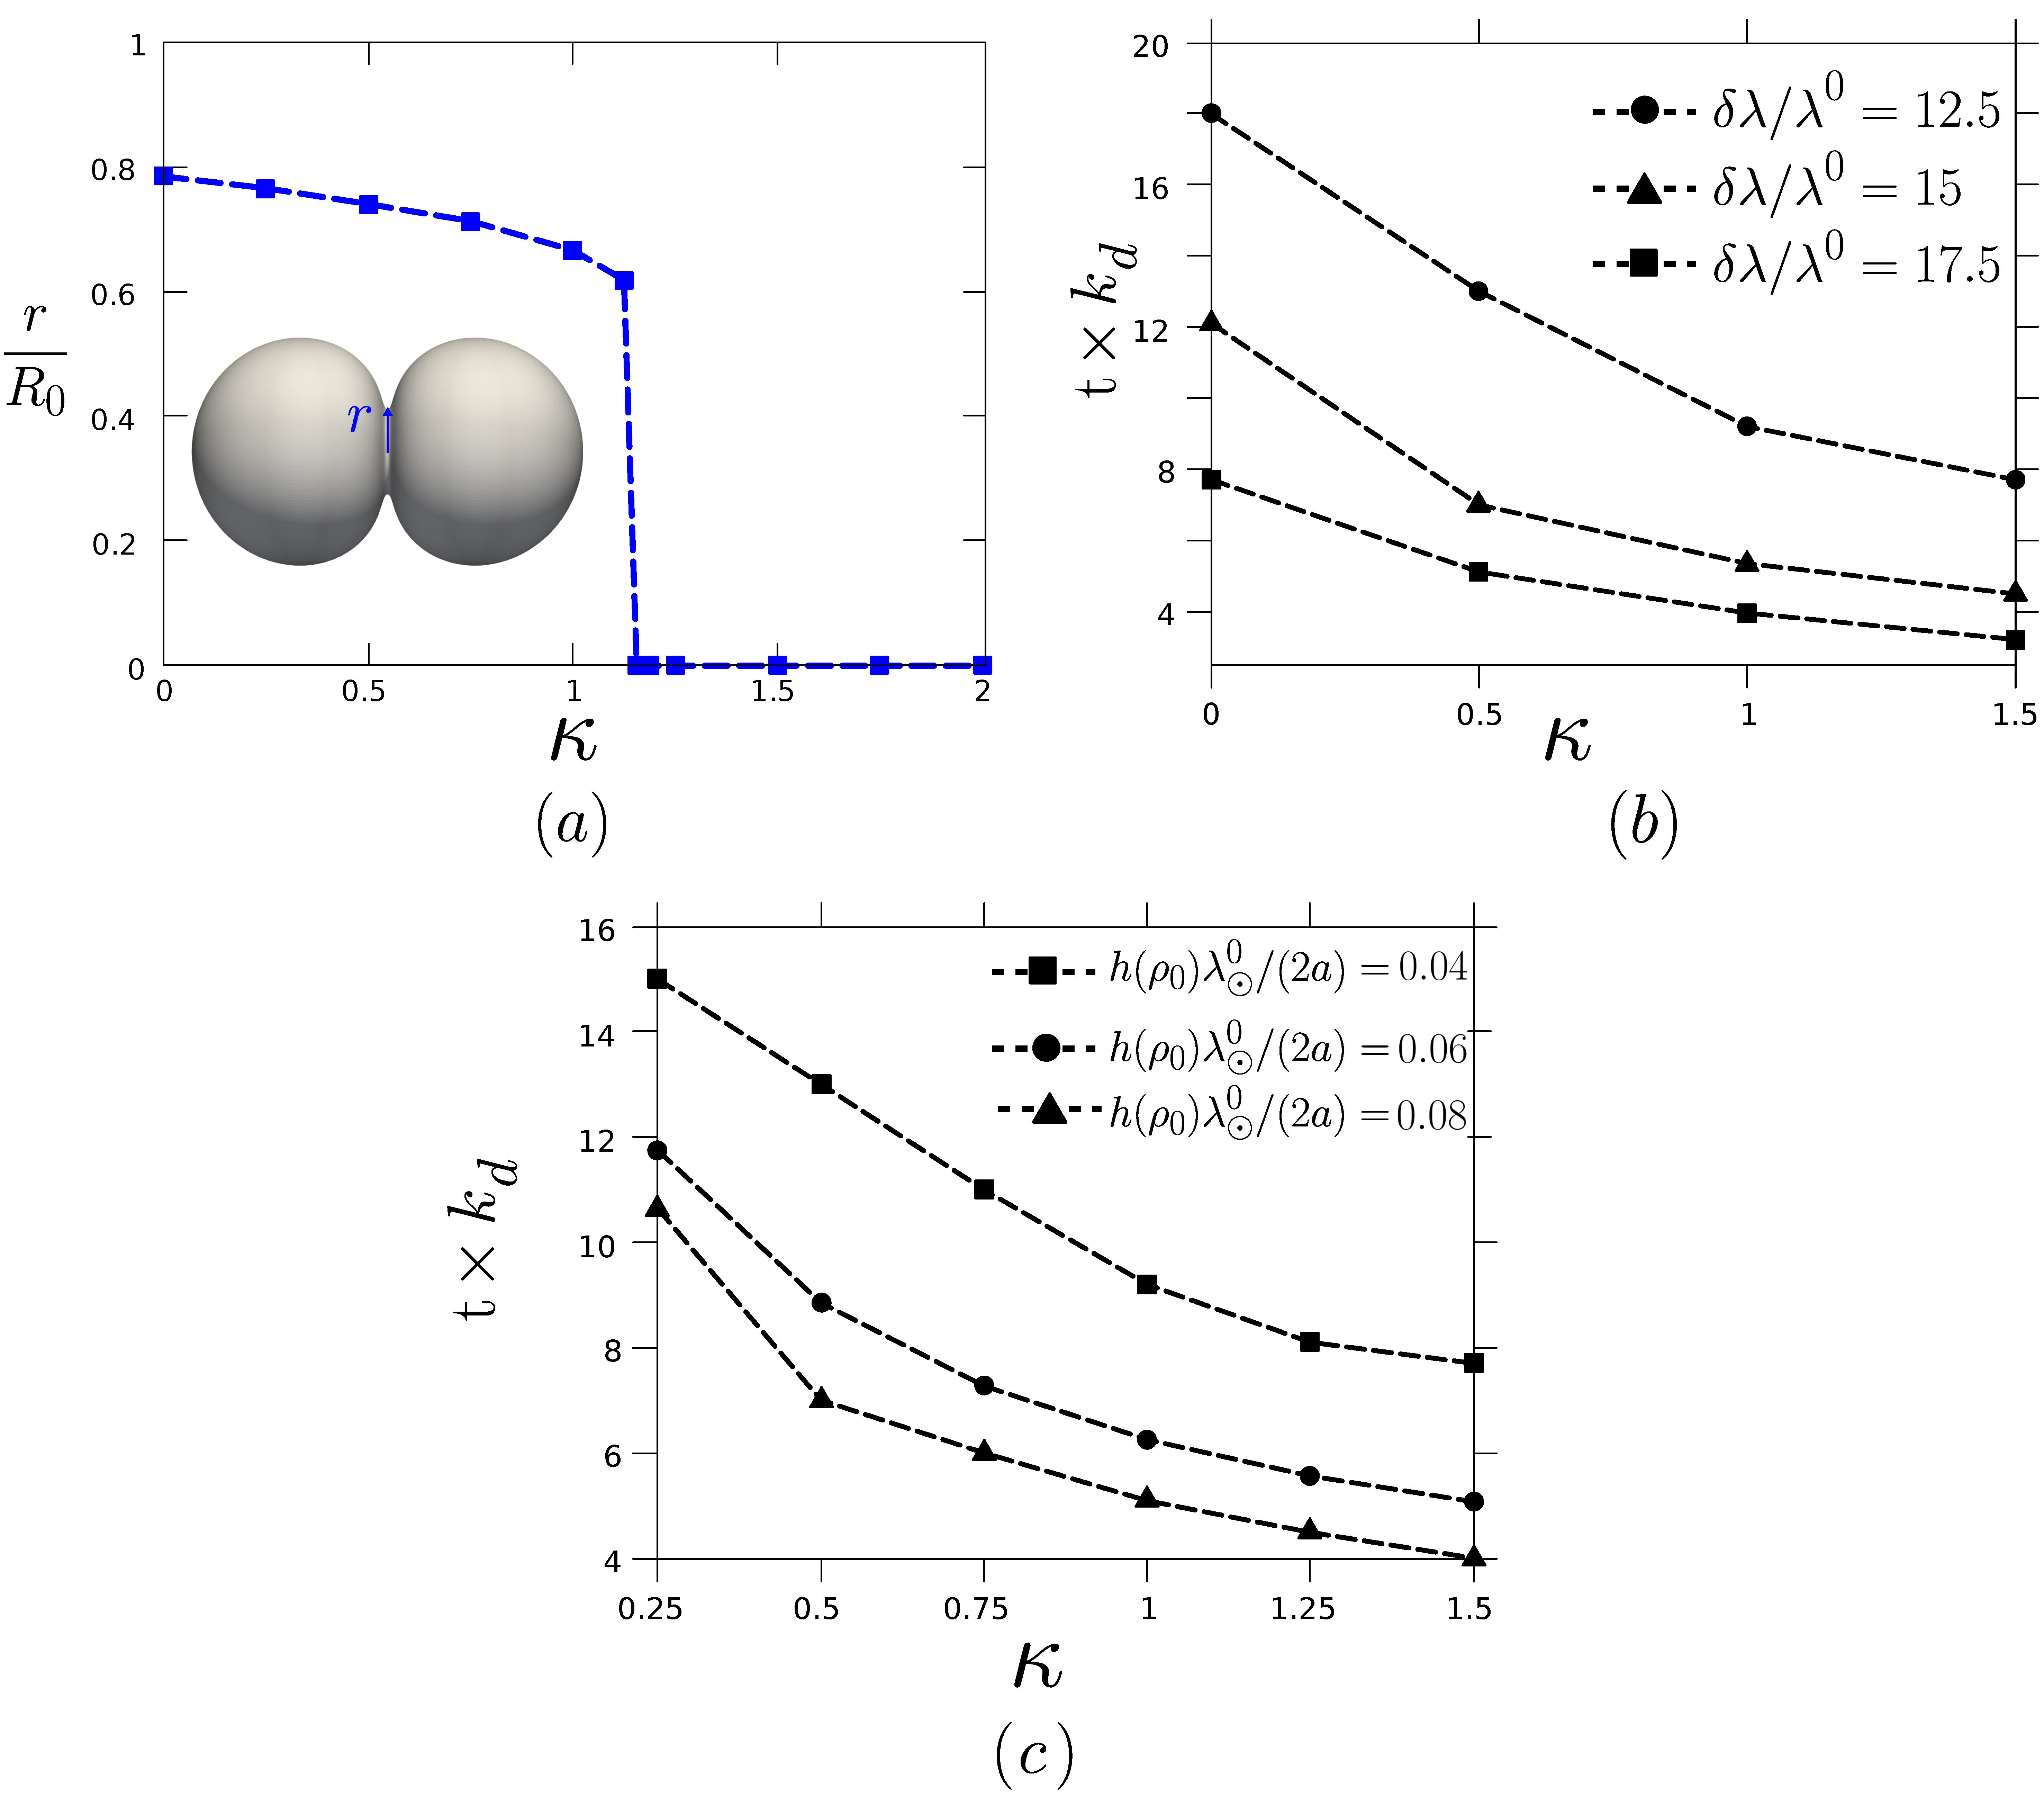
\includegraphics[width=0.8\textwidth]{chap_8_fig_3.pdf}
\caption{Influence of activity parameters on the cell division dynamics (a) Normalized final furrow radius as a function of tension anisotropy $\kappa = \lambda_{\rm aniso}/\lambda$ for a low over-activity $\delta\lambda/\lambda_0 = 10$, showing a threshold of $\kappa$ for full division. For larger over-activities considered in (b) and (c), full division takes place irrespective of $\kappa$.Time required for full division as a function of $\kappa$ for different over-activities (b) and for different active nematic forces (c). }
\label{fig_3_III}
\end{figure} 

We examined next how different model parameters affect the ability of the system to divide and the time required for the process to complete. We first considered a moderate over-activity $\delta\lambda/\lambda_0 = 10$ and plotted the final radius of the contracted furrow as we vary tension anisotropy $\kappa = \lambda_{\rm aniso}/\lambda$, Fig.~\ref{fig_3_III}(a). This figure shows a threshold of $\kappa$ below which full constriction fails. We then considered larger values of over-activity  $\delta\lambda/\lambda_0$ in the range 12.5 to 17.5, but much lower than that required for full division in the absence of nematic coupling, in the order of 45 \cite{turlier2014}. We found   that full division takes place irrespective of $\kappa$ but at a faster rate as $\kappa$ or over-activity increase, Fig.~\ref{fig_3_III}(b).  Finally, we tested the effect of  nematic activity $\lambda_{\odot}$, finding that this parameter also reduces the time required for division, Fig.~\ref{fig_3_III}(c). In summary, in addition to the previously identified role of over-activity \cite{turlier2014}, our results show that active tension anisotropy and nematic active forces, both induced by nematic order, significantly facilitate and accelerate division.


Finally, we examined the influence of the activity-saturation parameter $\rho_s$ in Eq.~(\ref{76_III}) on the dynamics of the system. For large $\rho_s$, $g(\rho)$ and $h(\rho)$ become constant and linear, respectively. The lack of saturation reduces the thresholds for full division and accelerates the process. %On the contrary, a non-monotonic activity-density relation, as described later in Eq.~(\ref{77_III}), increases the threshold and time required for division. 
However, irrespective of the activity-density relation, we found that  active tension anisotropy and nematic active forces enhance division.


\subsection{Division and polarization as self-organized symmetry-breaking modes}


\citet{mietke2019_2} have suggested, using linear stability analysis, that a spherical and uniform active gel can develop symmetry-breaking cytokinesis-like modes as a result of activity. To examine this possibility in a fully nonlinear regime, we considered zero equatorial over-activity and only  biased slightly the initial state with an equatorial density increase  of 1\%. For lower values of base activity $\lambda_0$, this perturbation was quickly erased due to turnover and diffusion. For high-enough $\lambda_0$, the system strongly enhanced the initial asymmetry and developed spontaneously the self-reinforcing mechanism strongly influenced by nematic order described in the previous Section~leading to cell division, Fig.~\ref{fig_8_III}. The shape of the neck region depends on value of the activity saturation density $\rho_s$. For saturating Hill's functions with $\rho_s = 1 ~\si{\micro \meter}$, the system develops long cylindrical necks of vanishing radius, Fig.~\ref{fig_8_III}(a) and \href{https://github.com/waleedmirzaPhD/movies_thesis.git}{Movie~7.2}, similar to those in \cite{mietke2019}. In the absence of saturation $\rho_s = \infty$, the system develops short and sharp necks instead, Fig.~\ref{fig_8_III}(b). 


\begin{figure}[h!]
\centering
\vspace*{0cm}\includegraphics[width=0.8\textwidth]{chap_8_fig_4.eps}
\caption{Self-organized constriction of a cell for (a) a saturated Hill's and a (b) non-saturating  dependence of activity on density. The snapshots show shape, density (colormap) and velocity (arrows), while the insets show nematic order. }
\label{fig_8_III}
\end{figure} 


\begin{figure}[h!]
\centering
\vspace*{0cm}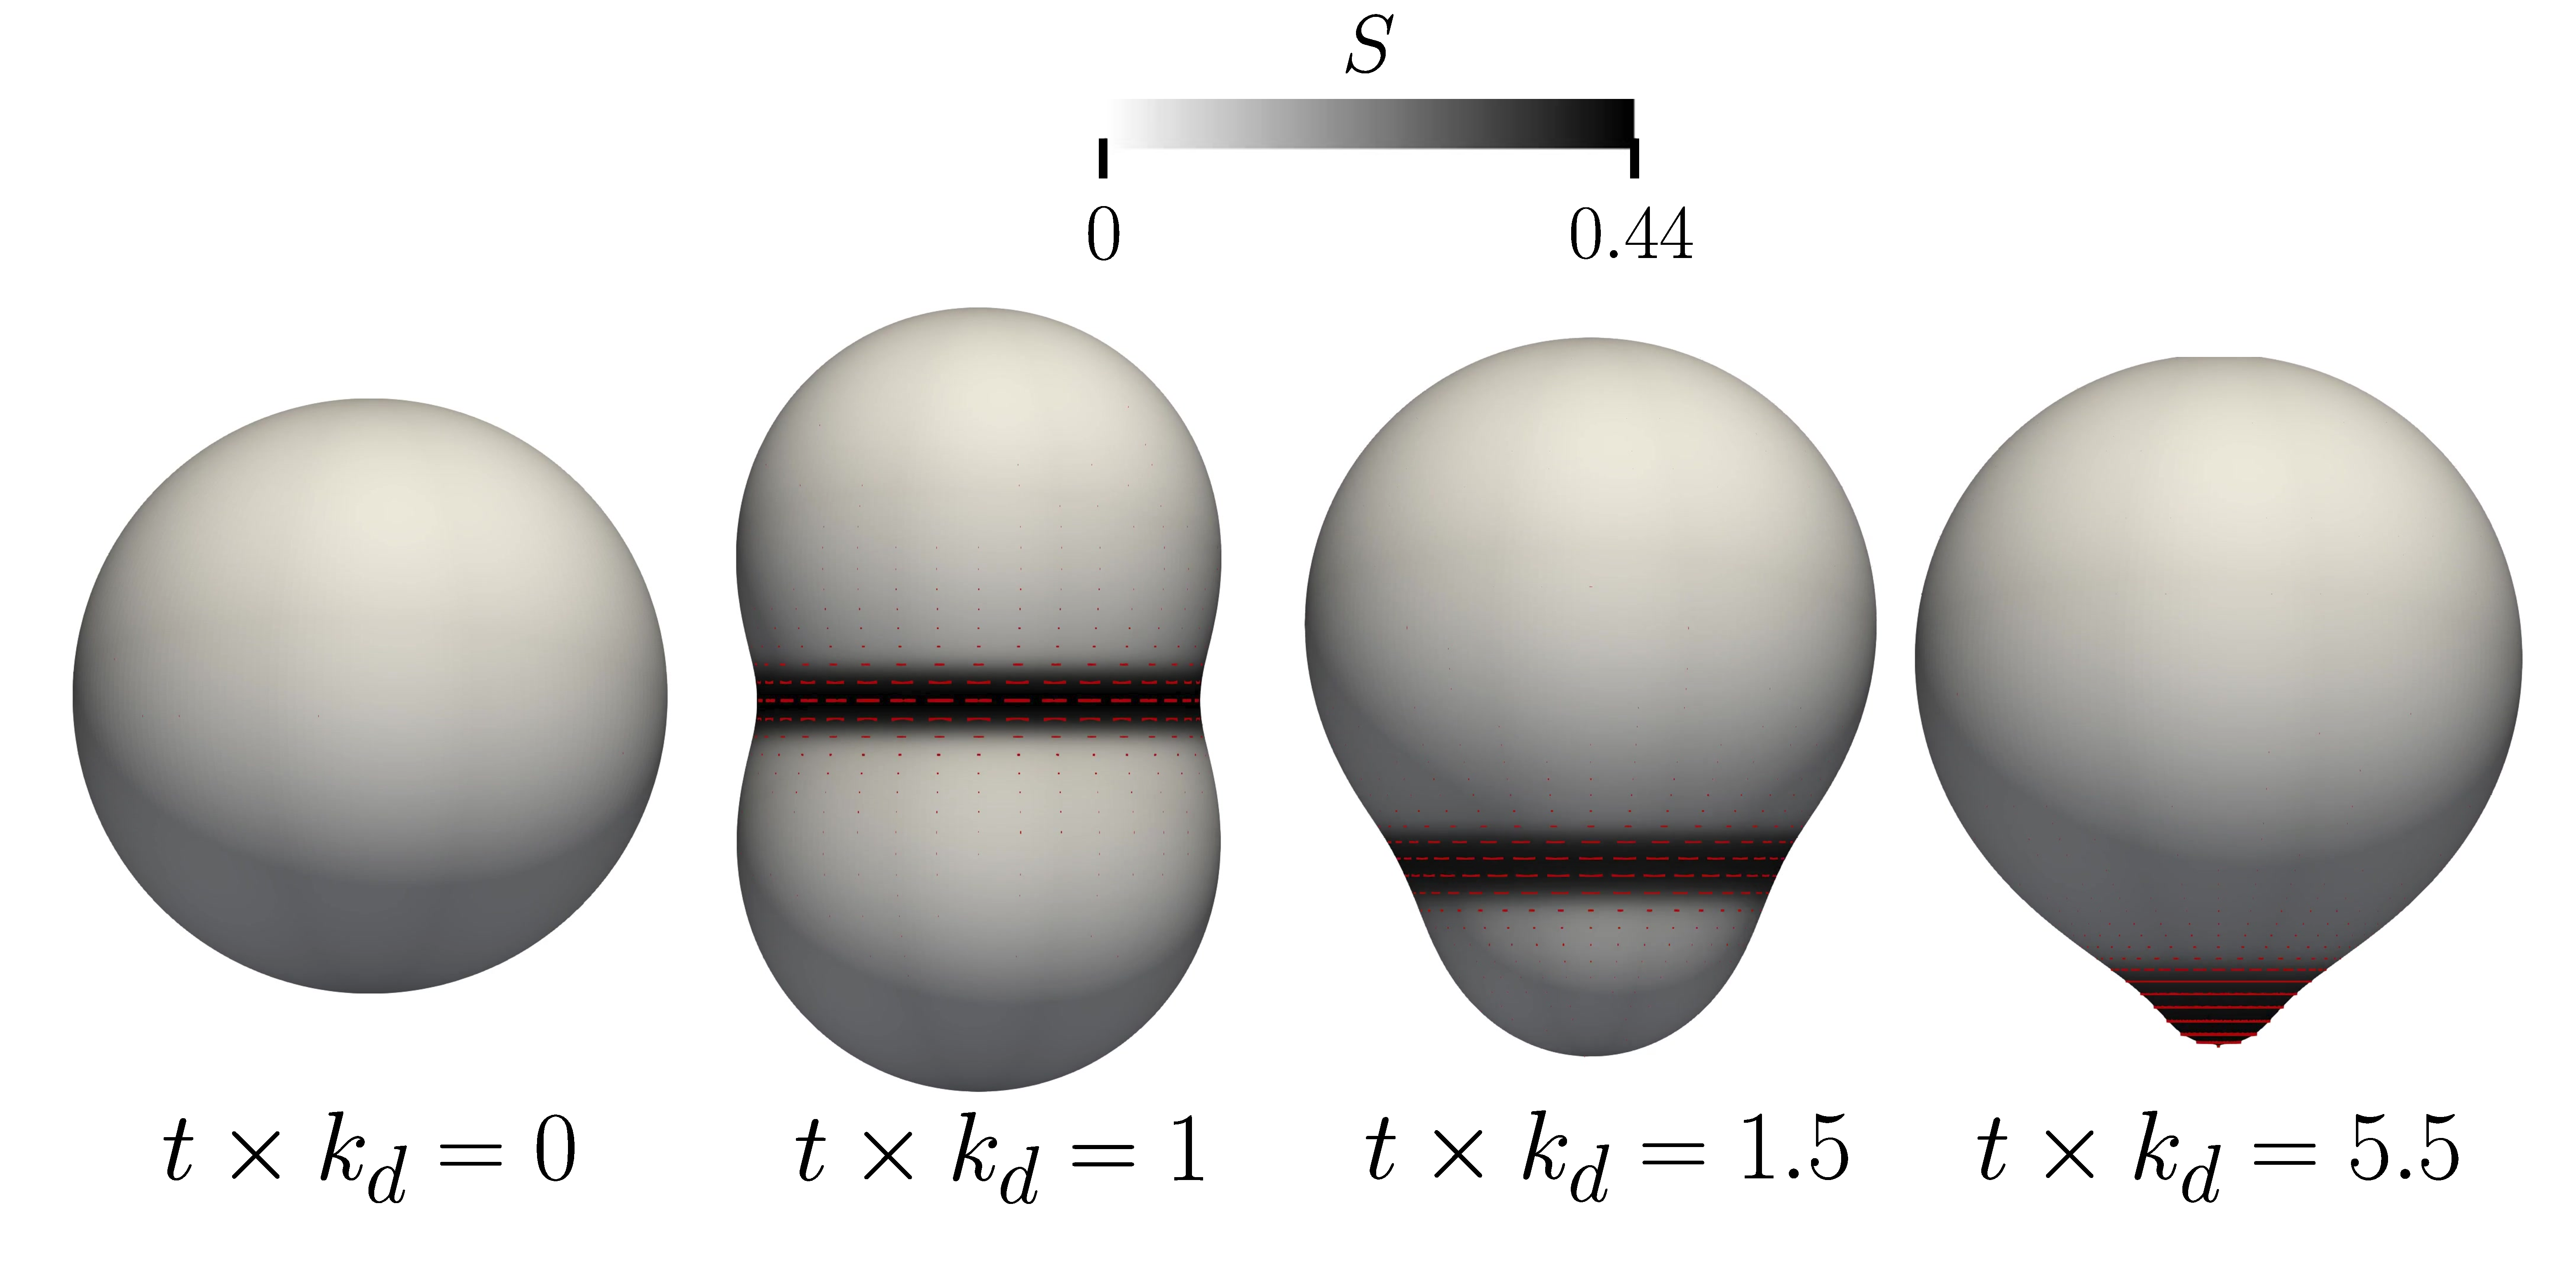
\includegraphics[width=0.65\textwidth]{chap_8_fig_5.pdf}
\caption{Spontaneous self-organization of a pseudoclevage furrow for no active  tension anisotropy, $\kappa = 0$, later evolving to a polarized ``cell migration'' mode.}
\label{fig_8.1_III}
\end{figure} 

Interestingly, for $\kappa=0$, the cytokinetic-like symmetry breaking mode is not strong enough to lead to full division and arrests in a pseudoclevage furrow configuration. Yet, at longer times, this state becomes unstable and further loses symmetry as the dense nematic ring slides towards one of the poles, eventually leading to a polarized state with sustained retrograde flow, Fig.~\ref{fig_8.1_III} and \href{https://github.com/waleedmirzaPhD/movies_thesis.git}{Movie~7.3}, akin to those observed in highly contractile non-adherent cells undergoing amoeboid motility \cite{Ruprecht:2015aa}.



One important difference between our simulations and the polarized cells observed by \citet{Ruprecht:2015aa} is the shape of the cell's rear. Whereas cortical density is highest in the rear both in experiments and simulations, the shape of cells suggests a complex active tension distribution, non-monotonic in density and possibly anisotropic. Independents studies in a different context also suggest a non-monotonic density-tension relation following experimental measurements \cite{chugh2017} or theoretical arguments  \cite{callan2013}. To examine this effect, we considered a non-monotonic dependence of active tension on density according to the functions 
\begin{equation} \label{77_III}
    g(\rho)  = 1-  \frac{1}{3} \left( \frac{\rho}{\rho_s}\right)^2,     h(\rho) = \rho-  \frac{\rho_s}{3} \left( \frac{\rho}{\rho_s}\right)^3
\end{equation}
such that, accounting for their density dependence, total active tension and active nematic force are $\lambda\left(\rho-  \frac{ \rho_s}{3} \left( \frac{\rho}{\rho_s}\right)^3 \right)$ and $\lambda_{\odot}\left(\rho^2-  \frac{\rho_s^2}{3} \left( \frac{\rho}{ \rho_s}\right)^4 \right)$ with maxima at $\sqrt{3}\rho_s$ \cite{torres2019, Ruprecht:2015aa}. 

\begin{figure}[H]
\centering
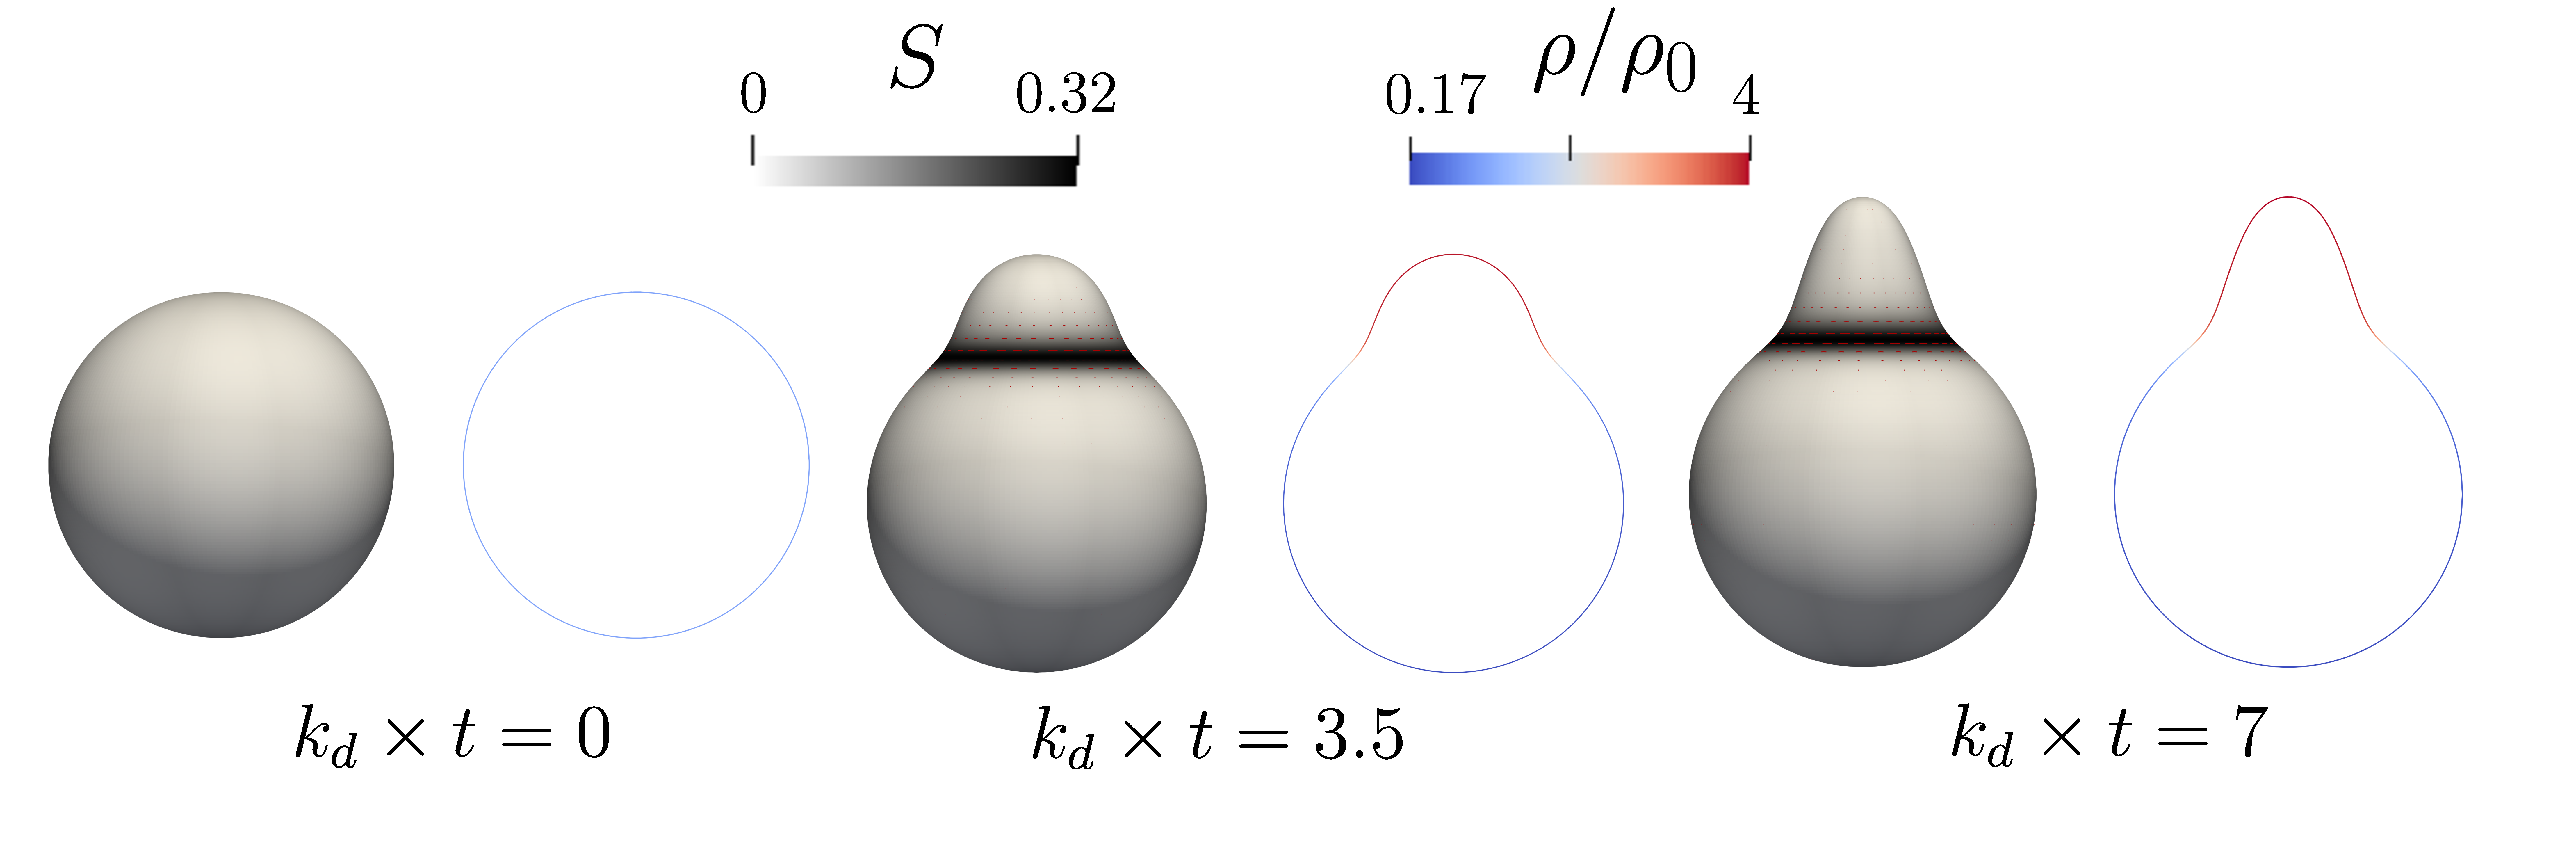
\includegraphics[width=\textwidth]{chap_8_fig_6.pdf}
\caption{Spontaneous self-organization of a polarized ``cell migration'' mode in an active gel with a non-monotonic dependence of active tension and nematic activity on cortical density.}
\label{fig_5_III}
\end{figure} 

To trigger the symmetry-breaking instability, we introduced in the initial state a random fluctuation in cortical density with maximum amplitude of 1\%. Above a threshold activity, the system develops a polarized ``cell-motility'' mode, Fig.~\ref{fig_5_III} and \href{https://github.com/waleedmirzaPhD/movies_thesis.git}{Movie~7.4}. The retrograde flow establishes a stable cortical density gradient towards the cell rear. As active tension and nematic activity are not a monotonic function of cortical thickness, their maxima  develop somewhere between the front and the rear of the cell, where a band of enhanced order develops. Since $\kappa>0$, this results in localized higher circumferential tension and pinching the cell into a pear shape. Thus, these results suggest that measurements of shape, cortical density and local nematic order in polarized cells may provide sufficient information to infer the dependence of active forces on density and filament alignment. %A parametric analysis of the influence of $\kappa$ on the cell shape (Fig.~\ref{fig_6_III} and Movie~$7.5$ in Appendix~\ref{appendix_2}) shows a higher value of anisotropic tension constricts the cell and creates  a thin tail-like protrusion in the rear of the cell.

%\begin{figure}[h!]
%\centering
%\vspace*{0cm}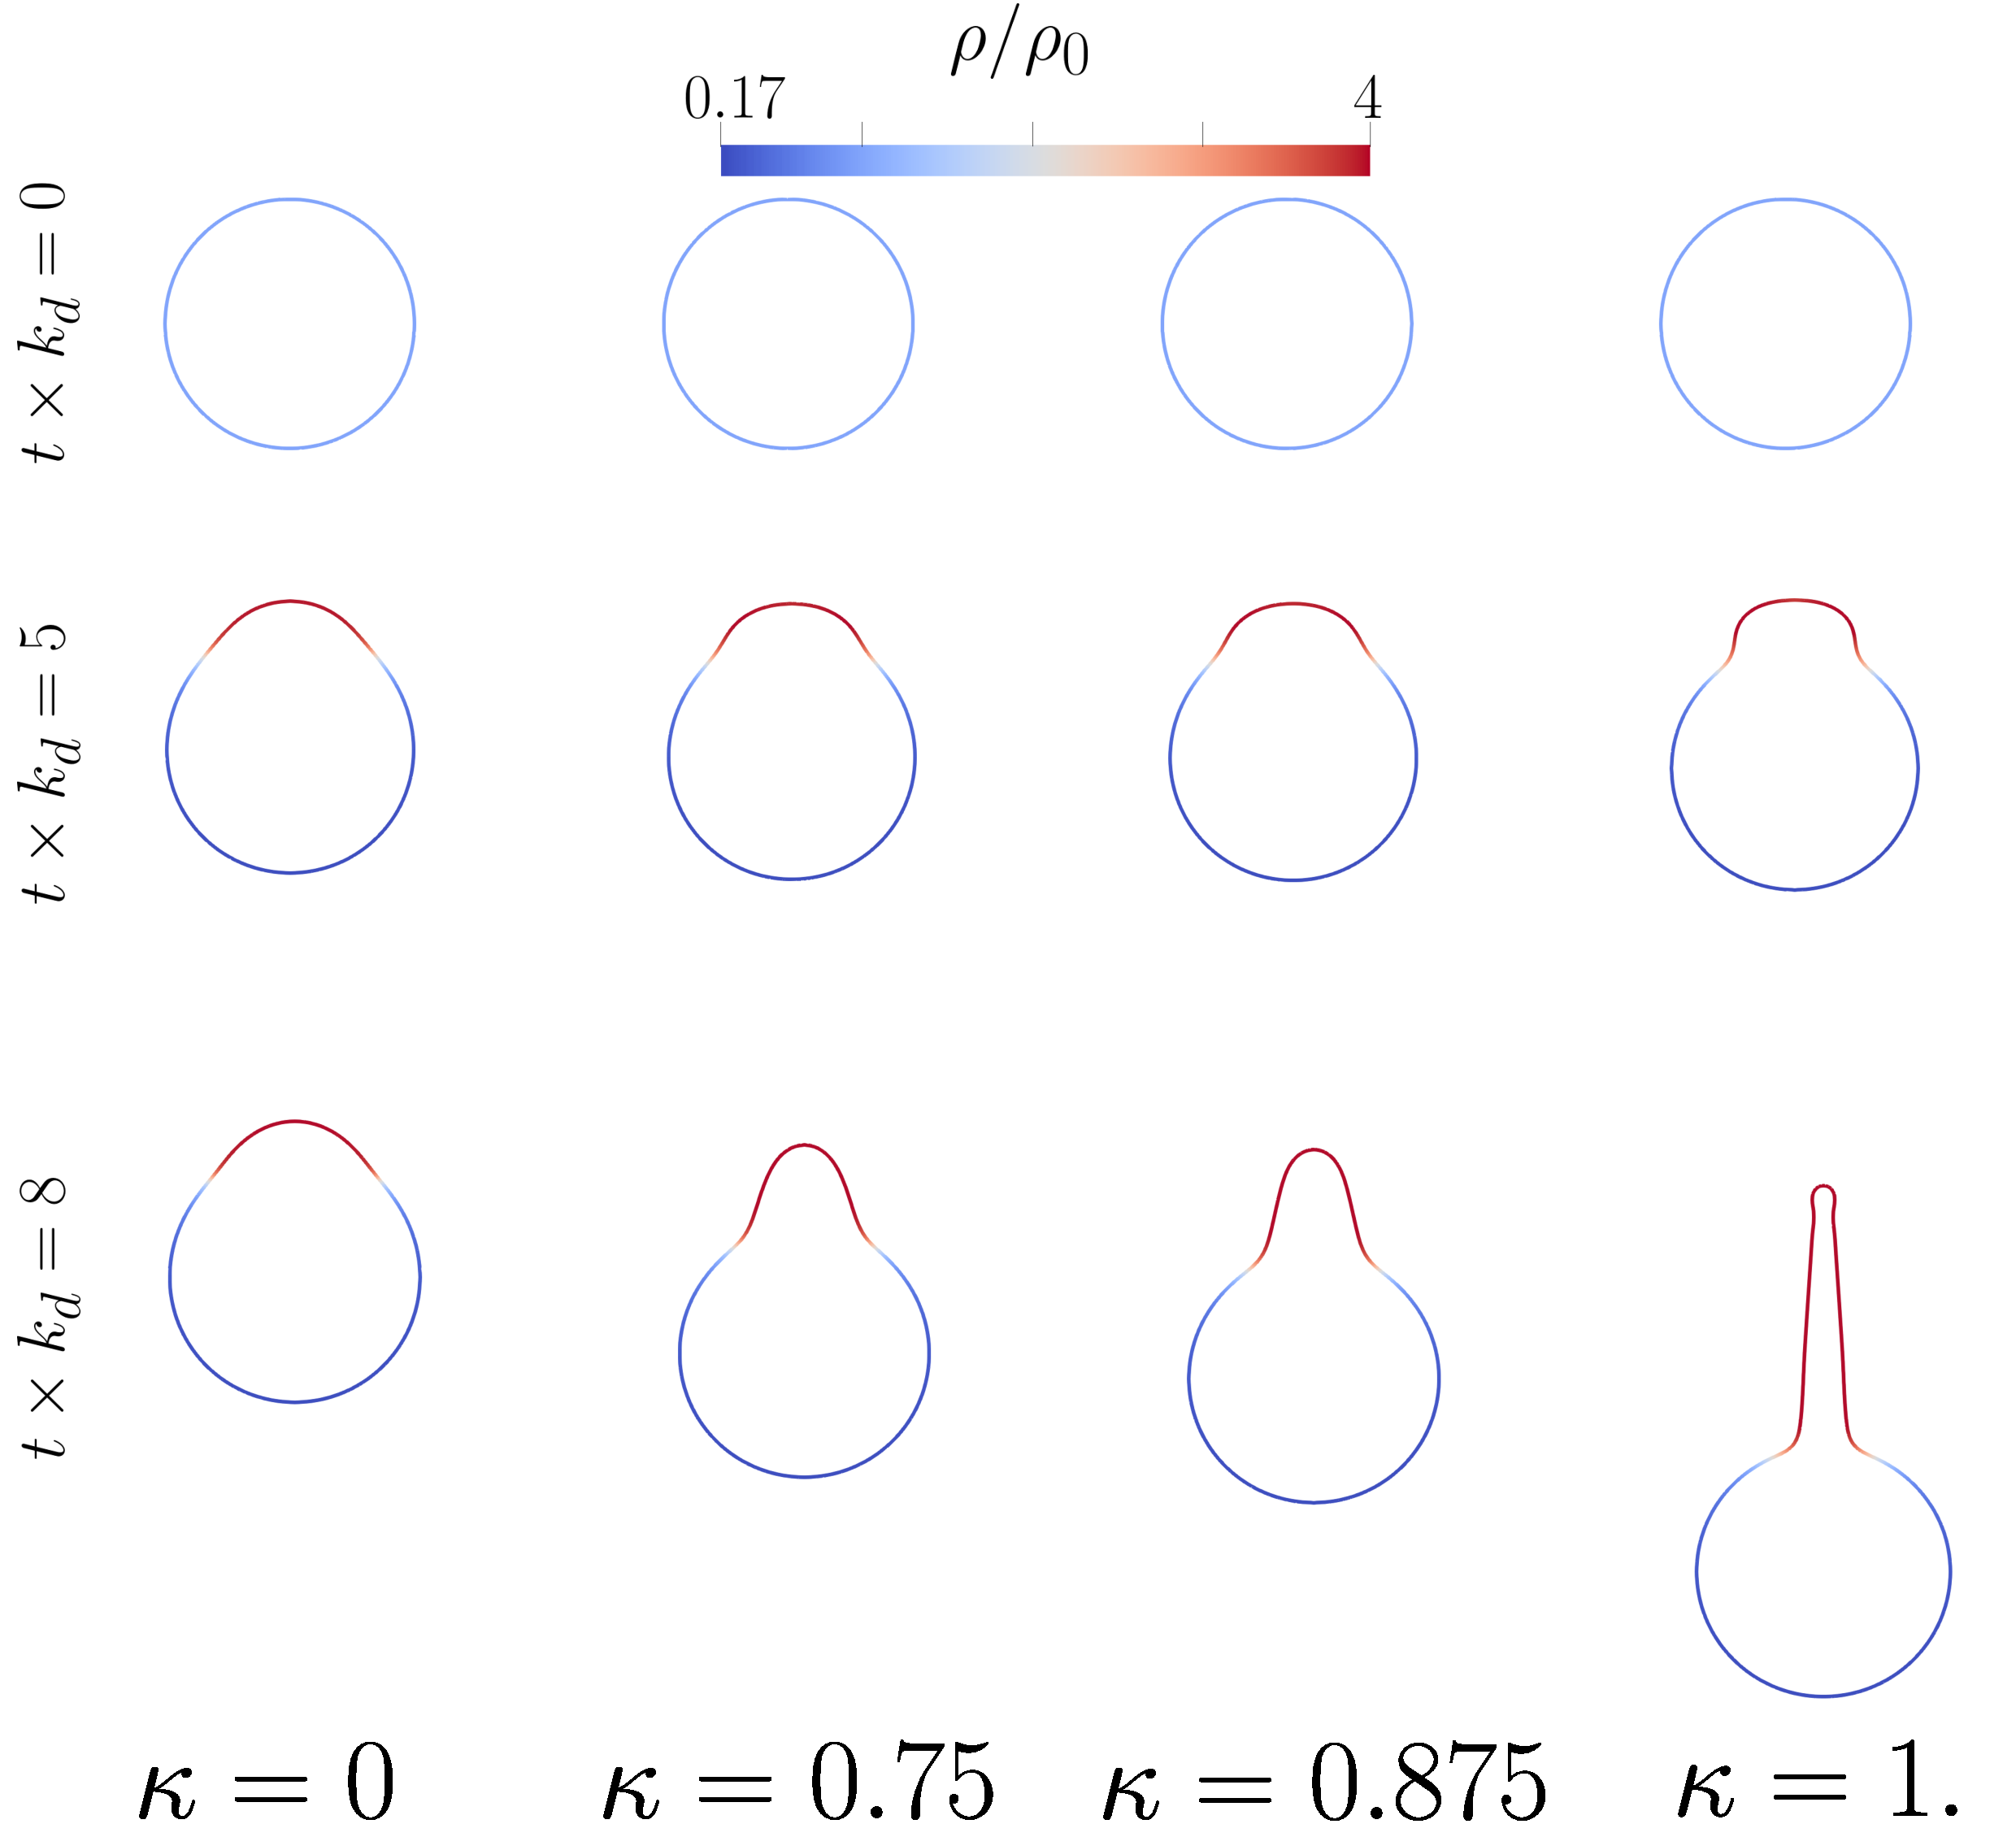
\includegraphics[width=1\textwidth]{chap_8_fig_7.pdf}
%\caption{Parametric analysis to demonstrate the influence of $\kappa$ on shape changes during cell motility. A higher value of $\kappa$ together with furrow ring-like actin architecture in the rear elongate the cell by creating constriction due to higher anisotropic contraction in the circumferential direction.}
%\label{fig_6_III}
%\end{figure} 


%The increased contractility introduces compressive hydrodynamic gradients which together with active torque align the network perpendicular to the axis of polarity forming the circumferential ring of actin network. For $\kappa>0$, the resulting anisotropy in architecture generates higher tension in circumferential direction in high-alignment region and hence locally pinching the cell into a pear shape. A parametric analysis of the influence of $\kappa$ on the cell shape (Fig.~\ref{fig_6_III} and \href{https://www.dropbox.com/s/aq3autc6uuefy2t/movie_2.3.4.mp4?dl=0}{Movie~$2.3.4$}) see Appendix~\ref{appendix_2} shows a higher value of anisotropic tension constricts the cell and creates  a thin tail-like protrusion in the rear of the cell. At higher active torque and contractility (Fig.~\ref{fig_7_III} and \href{https://www.dropbox.com/s/zdao6ix7kjil2rc/movie_2.3.5.mp4?dl=0}{Movie~$8.5$}) see Appendix~\ref{appendix_2} we observe an oscillatory motion of the tail-like protrusion whereby the rear end of the cell protrude and retract. As explained the protrusion results from higher anisotropic tension generated in the ring of actin network. This cell protrusion results in hydrodynamic extension in tail of the cell which locally aligns the fibers along the axis of polarity. This in turn allows the network to generate tension and retract the extrusion forward. The forward motion of the tail once again generates a compressive hydrodynamic gradient aligning fibers circumferentially and hence generating a sustained cycle of extrusion and retraction of the cell's rear-end. Lastly, it is imperative to reiterate that assuming contractility as linear or saturating Hill–Langmuir function of $\rho$ does not reproduce the shape changes or network architecture observed in \cite{Ruprecht:2015aa}.





%\begin{figure}[h!]
%\centering
%\vspace*{0cm}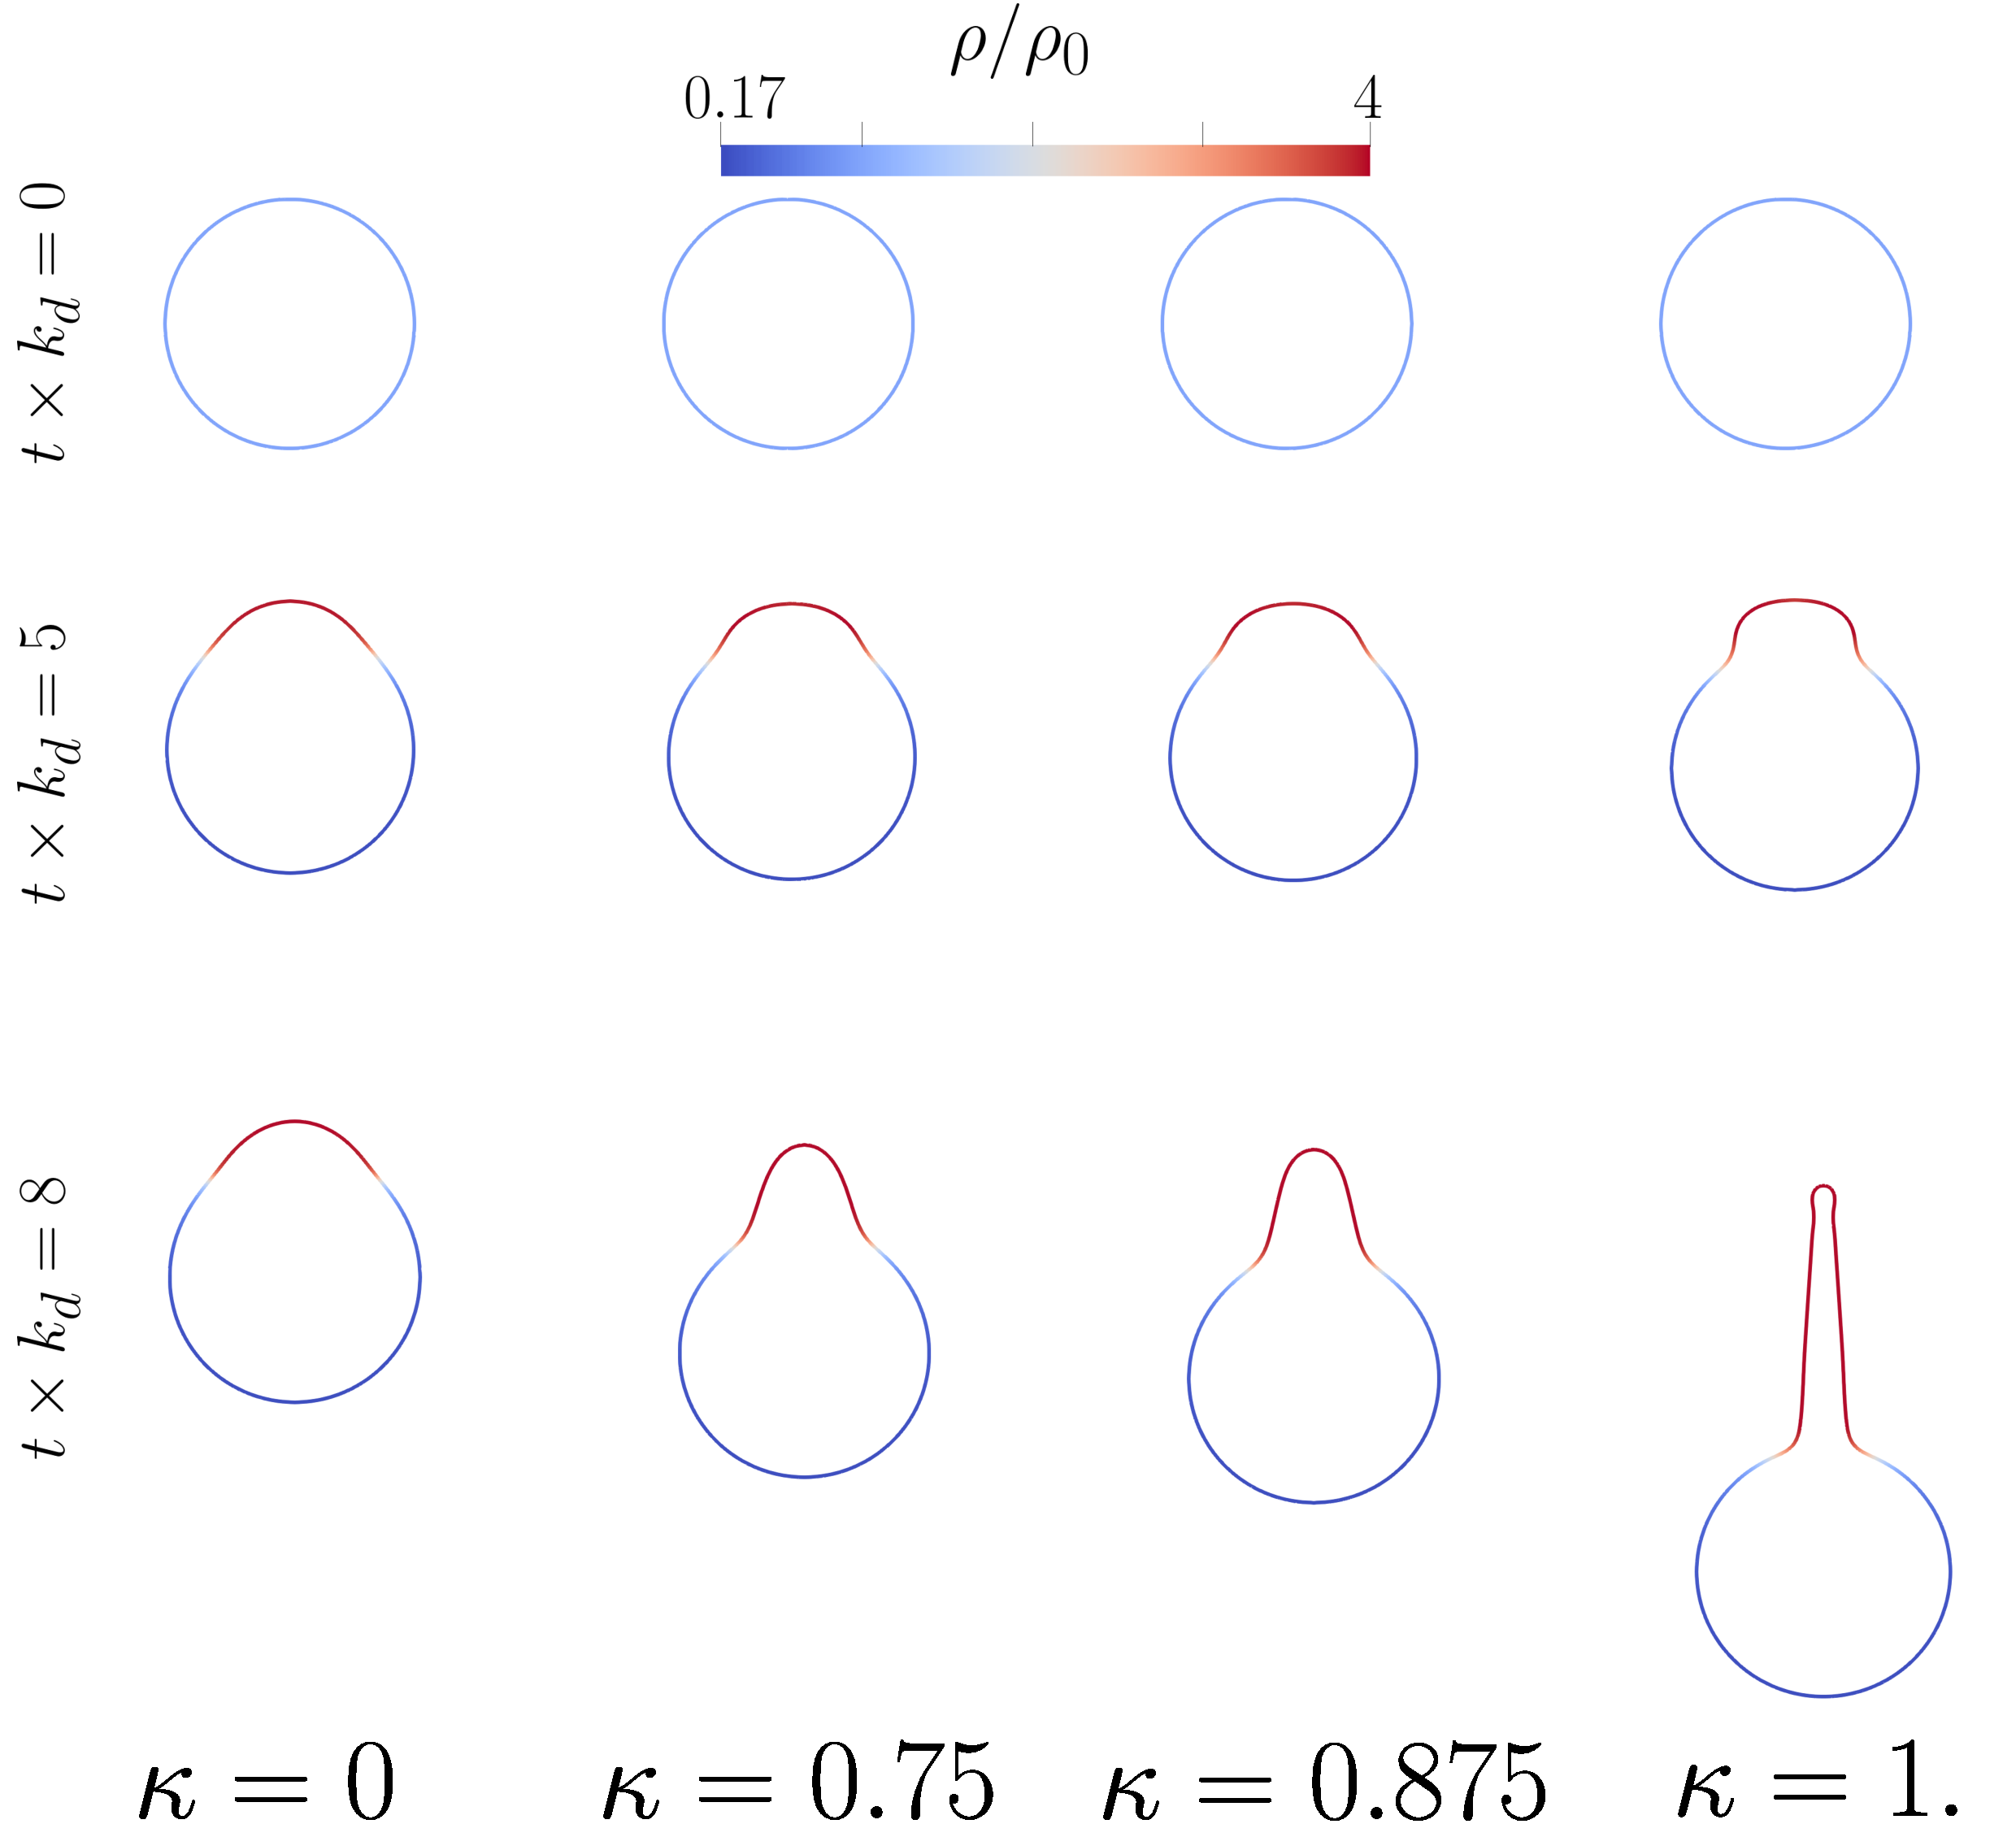
\includegraphics[width=1\textwidth]{chap_8_fig_7.pdf}
%\caption{Parametric analysis to demonstrate the influence of $\kappa$ on shape changes during cell motility. A higher value of $\kappa$ together with furrow ring-like actin architecture in the rear elongate the cell by creating constriction due to higher anisotropic contraction in the circumferential direction.}
%\label{fig_6_III}
%\end{figure} 
%
%\begin{figure}[h!]
%\centering
%\vspace*{0cm}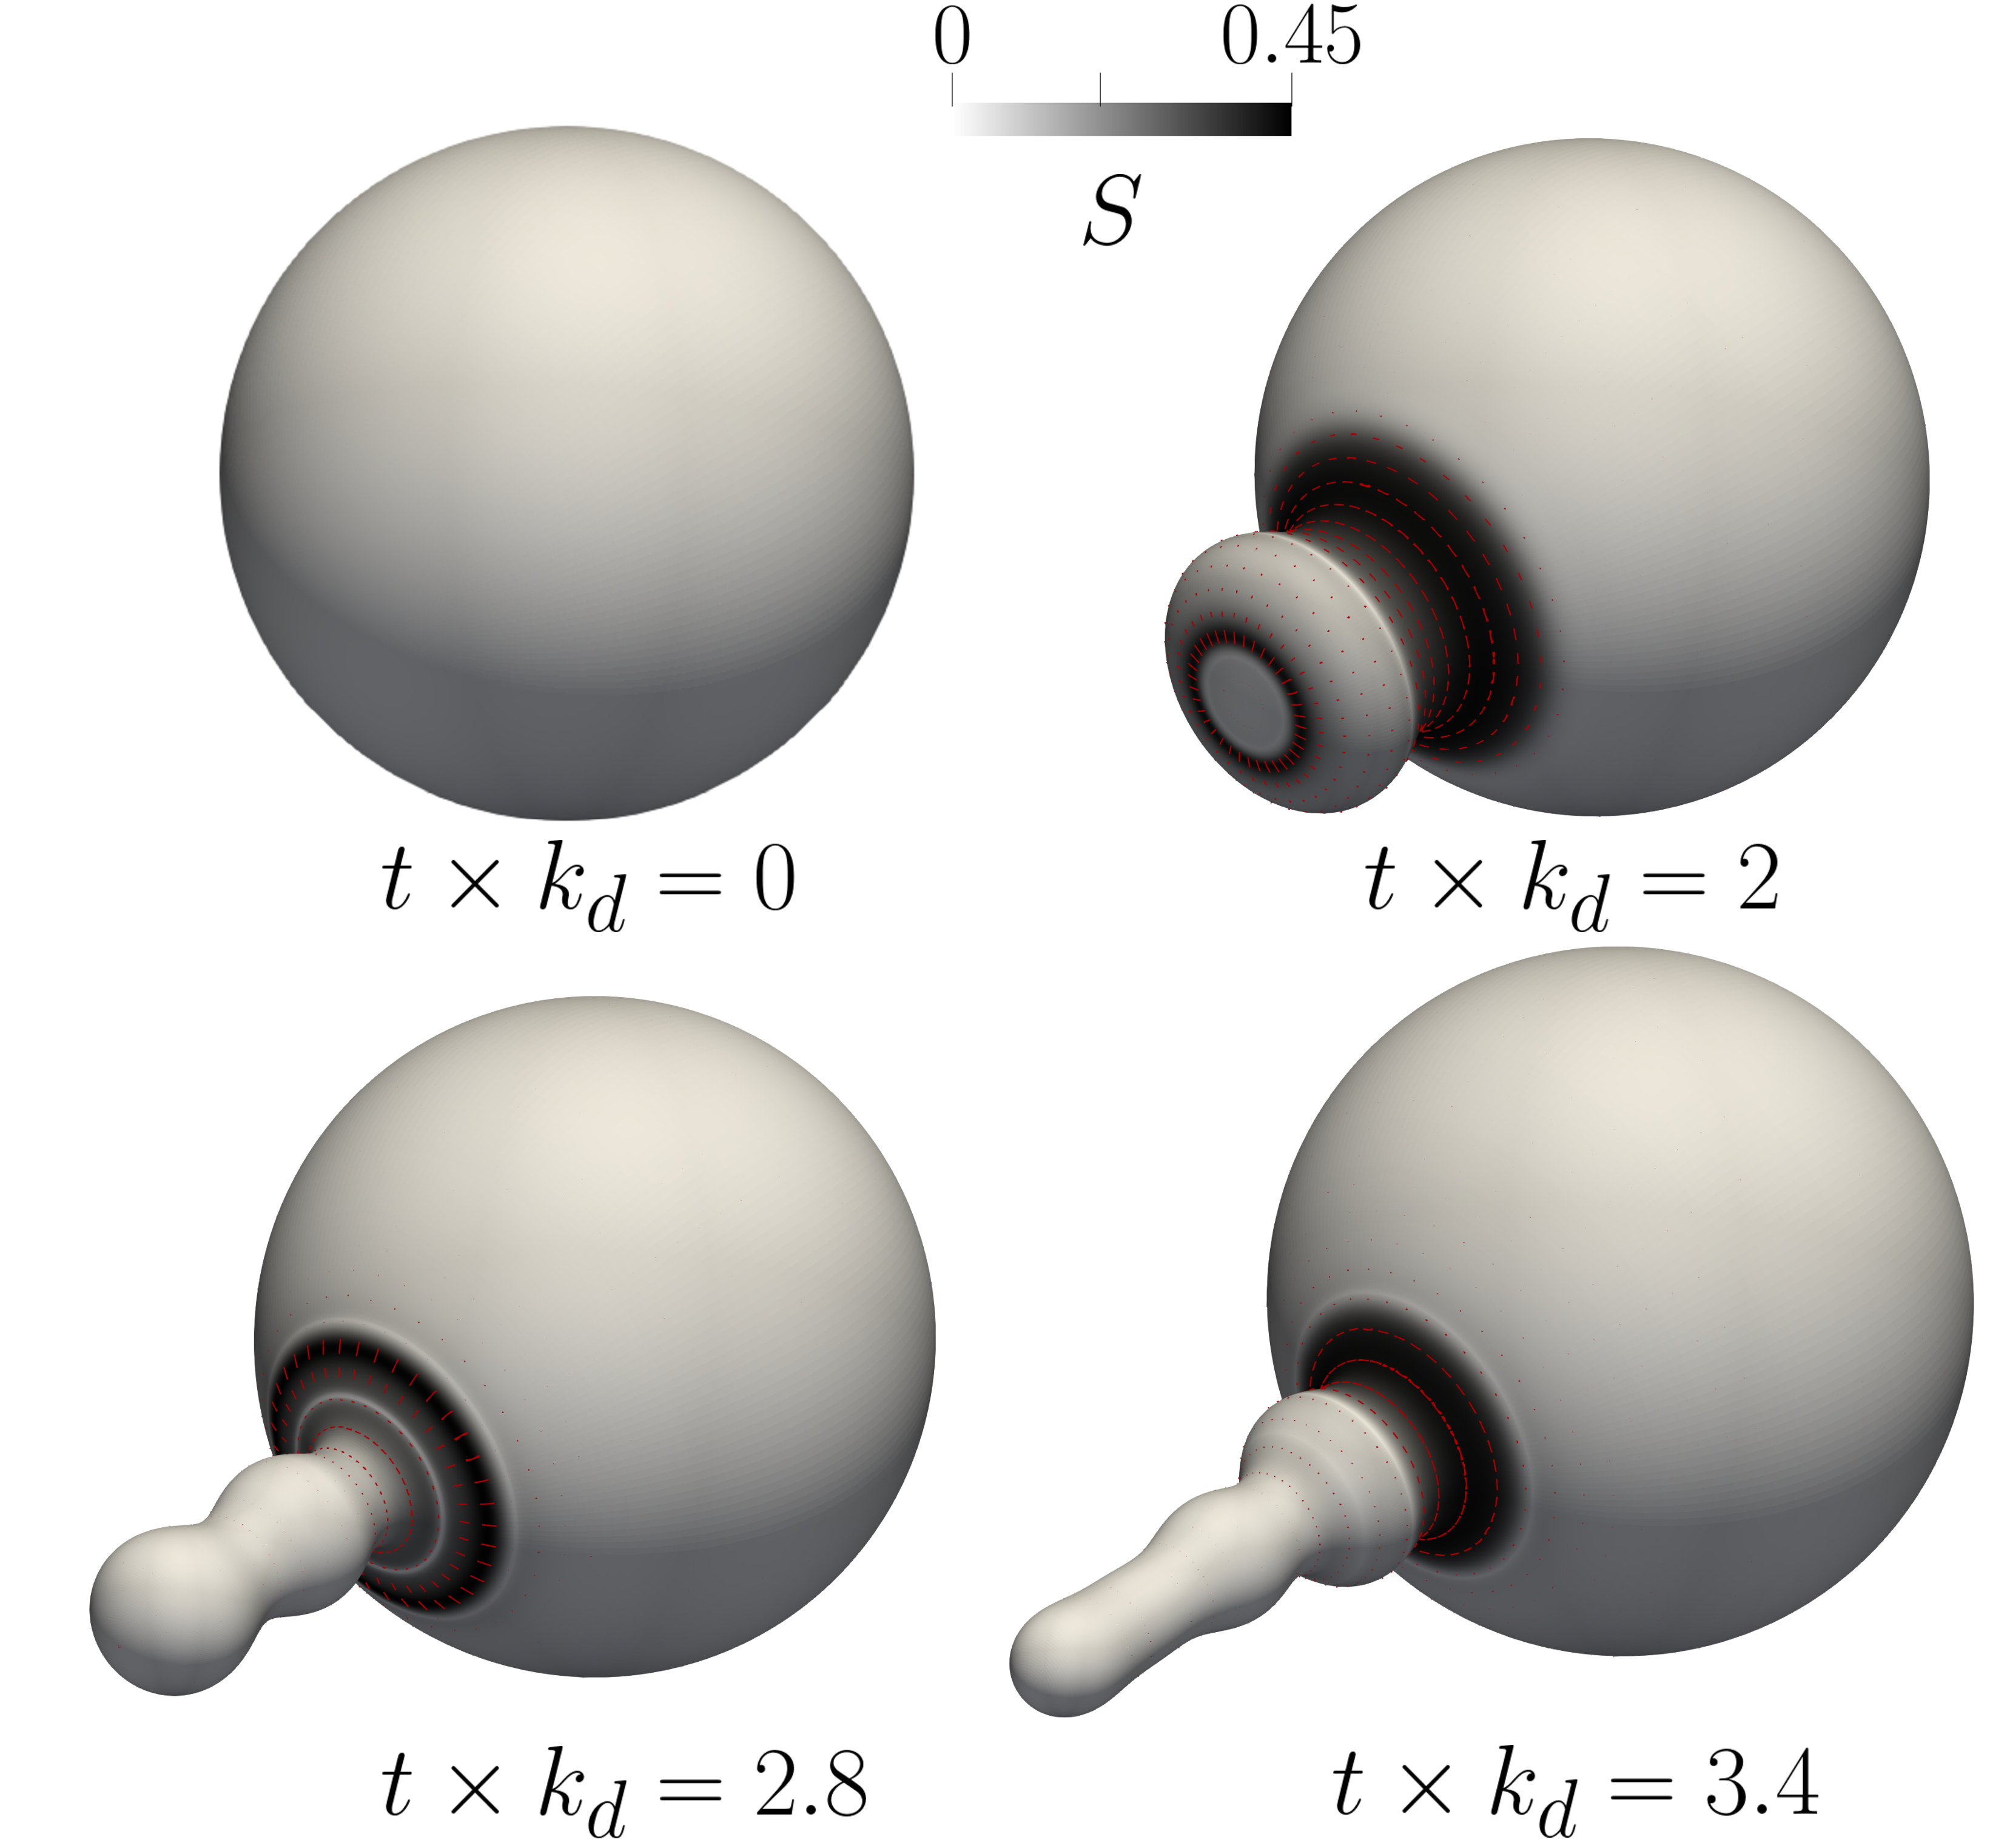
\includegraphics[width=0.8\textwidth]{chap_8_fig_8.pdf}
%\caption{Sequence of events involving self-organization of actin nematic architecture on a cortical surface due to a north-south pole symmetry breaking at a relatively higher activity of the bundling proteins. The shape changes result from an interplay between actin flow to the rear of the cell and periodic oscillations of actin network alignment between the polarity axis and in the normal direction to the polarity axis. The length and direction of the red segment indicate nematic order parameter $S$ and $\bm{n}$ respectively. Movie~corresponding to this figure can be accessed here \href{https://www.dropbox.com/s/zdao6ix7kjil2rc/movie_2.3.5.mp4?dl=0}{movie~$8.5$} see Appendix~\ref{appendix_2}}
%\label{fig_7_III}
%\end{figure} 




\section{Summary}

In this chapter, we have particularized the theory for active nematic gels on deformable surfaces proposed in Chapter~\ref{chap_7} to axisymmetry. We have also developed a fully discrete numerical formulation based on a time-incremental Onsager principle and a B-Spline finite element discretization. This approach grants very fast fully nonlinear simulations of the dynamics coupling  cytoskeletal density, nematic order, and surface shape. We have focused on cell division and polarized cellular states, for which axisymmetry is a reasonable assumption.

Our results support the notion that increased equatorial contractility leads to the self-organization of a high-density band with high alignment that efficiently constricts the cell \cite{anne2016}. Our results further show that the nematic coupling significantly affects previous results about the biophysics of cell division. More specifically, we find that nematic coupling reduces the threshold of equatorial over-activity required to complete division, and significantly accelerates the process. Furthermore, in the absence of equatorial over-activity, we show in the fully nonlinear regime that beyond a base activity, the system develops a symmetry-breaking cytokinetic-like instability leading to cell division as previously suggested \cite{mietke2019_2}. Thus, on top of biologically controlled equatorial  overactivity \cite{spira2017}, self-organization can contribute to robust cell division. We also show that our model can develop polarized motility-like instabilities with cellular shapes similar to those  observed experimentally \cite{Ruprecht:2015aa} that depend on how active tension is modulated by density and nematic order. 

%Lastly, the solution of the proposed model in the axisymmetric setting is very limited in terms of exploring relevant biological systems. The literature review in Chapter~(\ref{chap_6}) indicates that several biological surfaces such as a vesicle or an epithelial layer do not abide by the constraint of axisymmetry and hence the dependence on the coordinate $\varphi$ arises. Therefore, in the next chapter, we proposed the numerical solution of the model on an arbitrary manifold and explore it in the relevant settings.





